%!TEX root = ../thesis.tex
\chapter{Analyse von Build- und Deployment-Anwendungen}

Vor der Umsetzung der Anwendung wurde eine Analyse vorhandener Systeme durchgeführt. Die Ausarbeitung der Gemeinsamkeiten, Unterschiede, Vor- und Nachteile dieser Anwendungen helfen bei der Umsetzung der eigenen Anwendung.

Besonders Vor- und Nachteile sind subjektiv und unterscheiden sich zwischen Nutzergruppen. Bei der Betrachtung über Personae können diese Eigenschaften auf verschiedene Nutzergruppen projiziert werden.

Da der Fokus der Arbeit auf der Umsetzung liegt, wird die Analyse nur verkürzt durchgeführt, anhand der drei Anwendungen Jenkins, Travis CI und Codeship mit einer Persona. Die Anwendungen wurden aufgrund ihrere Bekanntheit und unterschiedlichen Herangehensweisen gewählt.

Zum Testen wurde jeweils eine Pipeline konfiguriert und mehrere Build-Prozesse nacheinander ausgelöst. Dabei wurden alle Anwendungen so benutzt, wie sie Out-of-the-box angeboten werden, ohne Erweiterungen oder externe Hilfsmittel.

\section{Persona}

Folgende Persona wurde zur Analyse genutzt:

\begin{figure}[h]
  \caption{Persona: Christian Köhler}
  \label{fig:persona}
  
\includegraphics[width=6cm]{assets/persona}
  \floatfoot{Foto von Elijah Henderson, lizenziert unter Creative Commons 2.0}
\end{figure}

\begin{description}
  \item [Name] Christian Köhler
  \item [Alter] 27 Jahre
  \item [Geschlecht] Männlich
  \item [Wohnort] Hamburg, Deutschland
  \item [Interessen] Internet, neue Technologien, Open Source, Indie-Filme
  \item [Abschluss] Informatik B. Sc.
  \item [Beruf] Freiberuflicher Softwareentwickler von Webanwendungen
  \item [Biografie] Christian hat Informatik studiert und dort seine Interesse an moderner Webentwicklung entdeckt. Im Studium hat er als freiberuflich Webentwickler gearbeitet und dies nach dem Studium fortgesetzt. In seiner Freizeit entwickelt und unterstützt er Open Source Projekte. Christian möchte einen eigenen Online-Dienst entwickeln, dafür aber vorerst nicht viel Geld investieren. Als Abwechslung vom Programmieren schaut er Kurzfilme aus der Indie-Szene.
  \item [Bedürfnis] Sowohl für seine freiberufliche Tätigkeit als auch für seine Projekte in der Freizeit sucht Christian eine Möglichkeit, um Webanwendungen automatisiert auf einen Server zu übertragen. Christian arbeitet mit Git. Zum Deployment führt er meist manuell auf dem Server einen \texttt{git pull} aus, womit er nicht zufrieden ist.
\end{description}

\section{Jenkins}
\label{sec:analyse-jenkins}

Jenkins ist eine in Java programmierte Webanwendung für Build-Prozesse. Es bezeichnet sich selbst als ``the leading open source automation server''\footnote{Quelle: https://jenkins.io/}. Jenkins ist ein Fork von Hudson, welches 2005 veröffentlicht wurde, mittlerweile aber nicht mehr weiterentwickelt wird. Jenkins ist kostenlos und muss selbst gehosted werden.

Es lässt sich mit vielen Plugins erweitern, was in diesem Szenario nicht berücksichtigt wurde.

Zur Analyse wurde Jenkins auf einer Serverinstanz installiert. Durch das angebotene Installationsskript war die Installation unkompliziert.

\begin{figure}[h]
  \caption{Jenkins: Konfiguration einer Pipeline}
  \label{fig:jenkins-pipeline-config}
  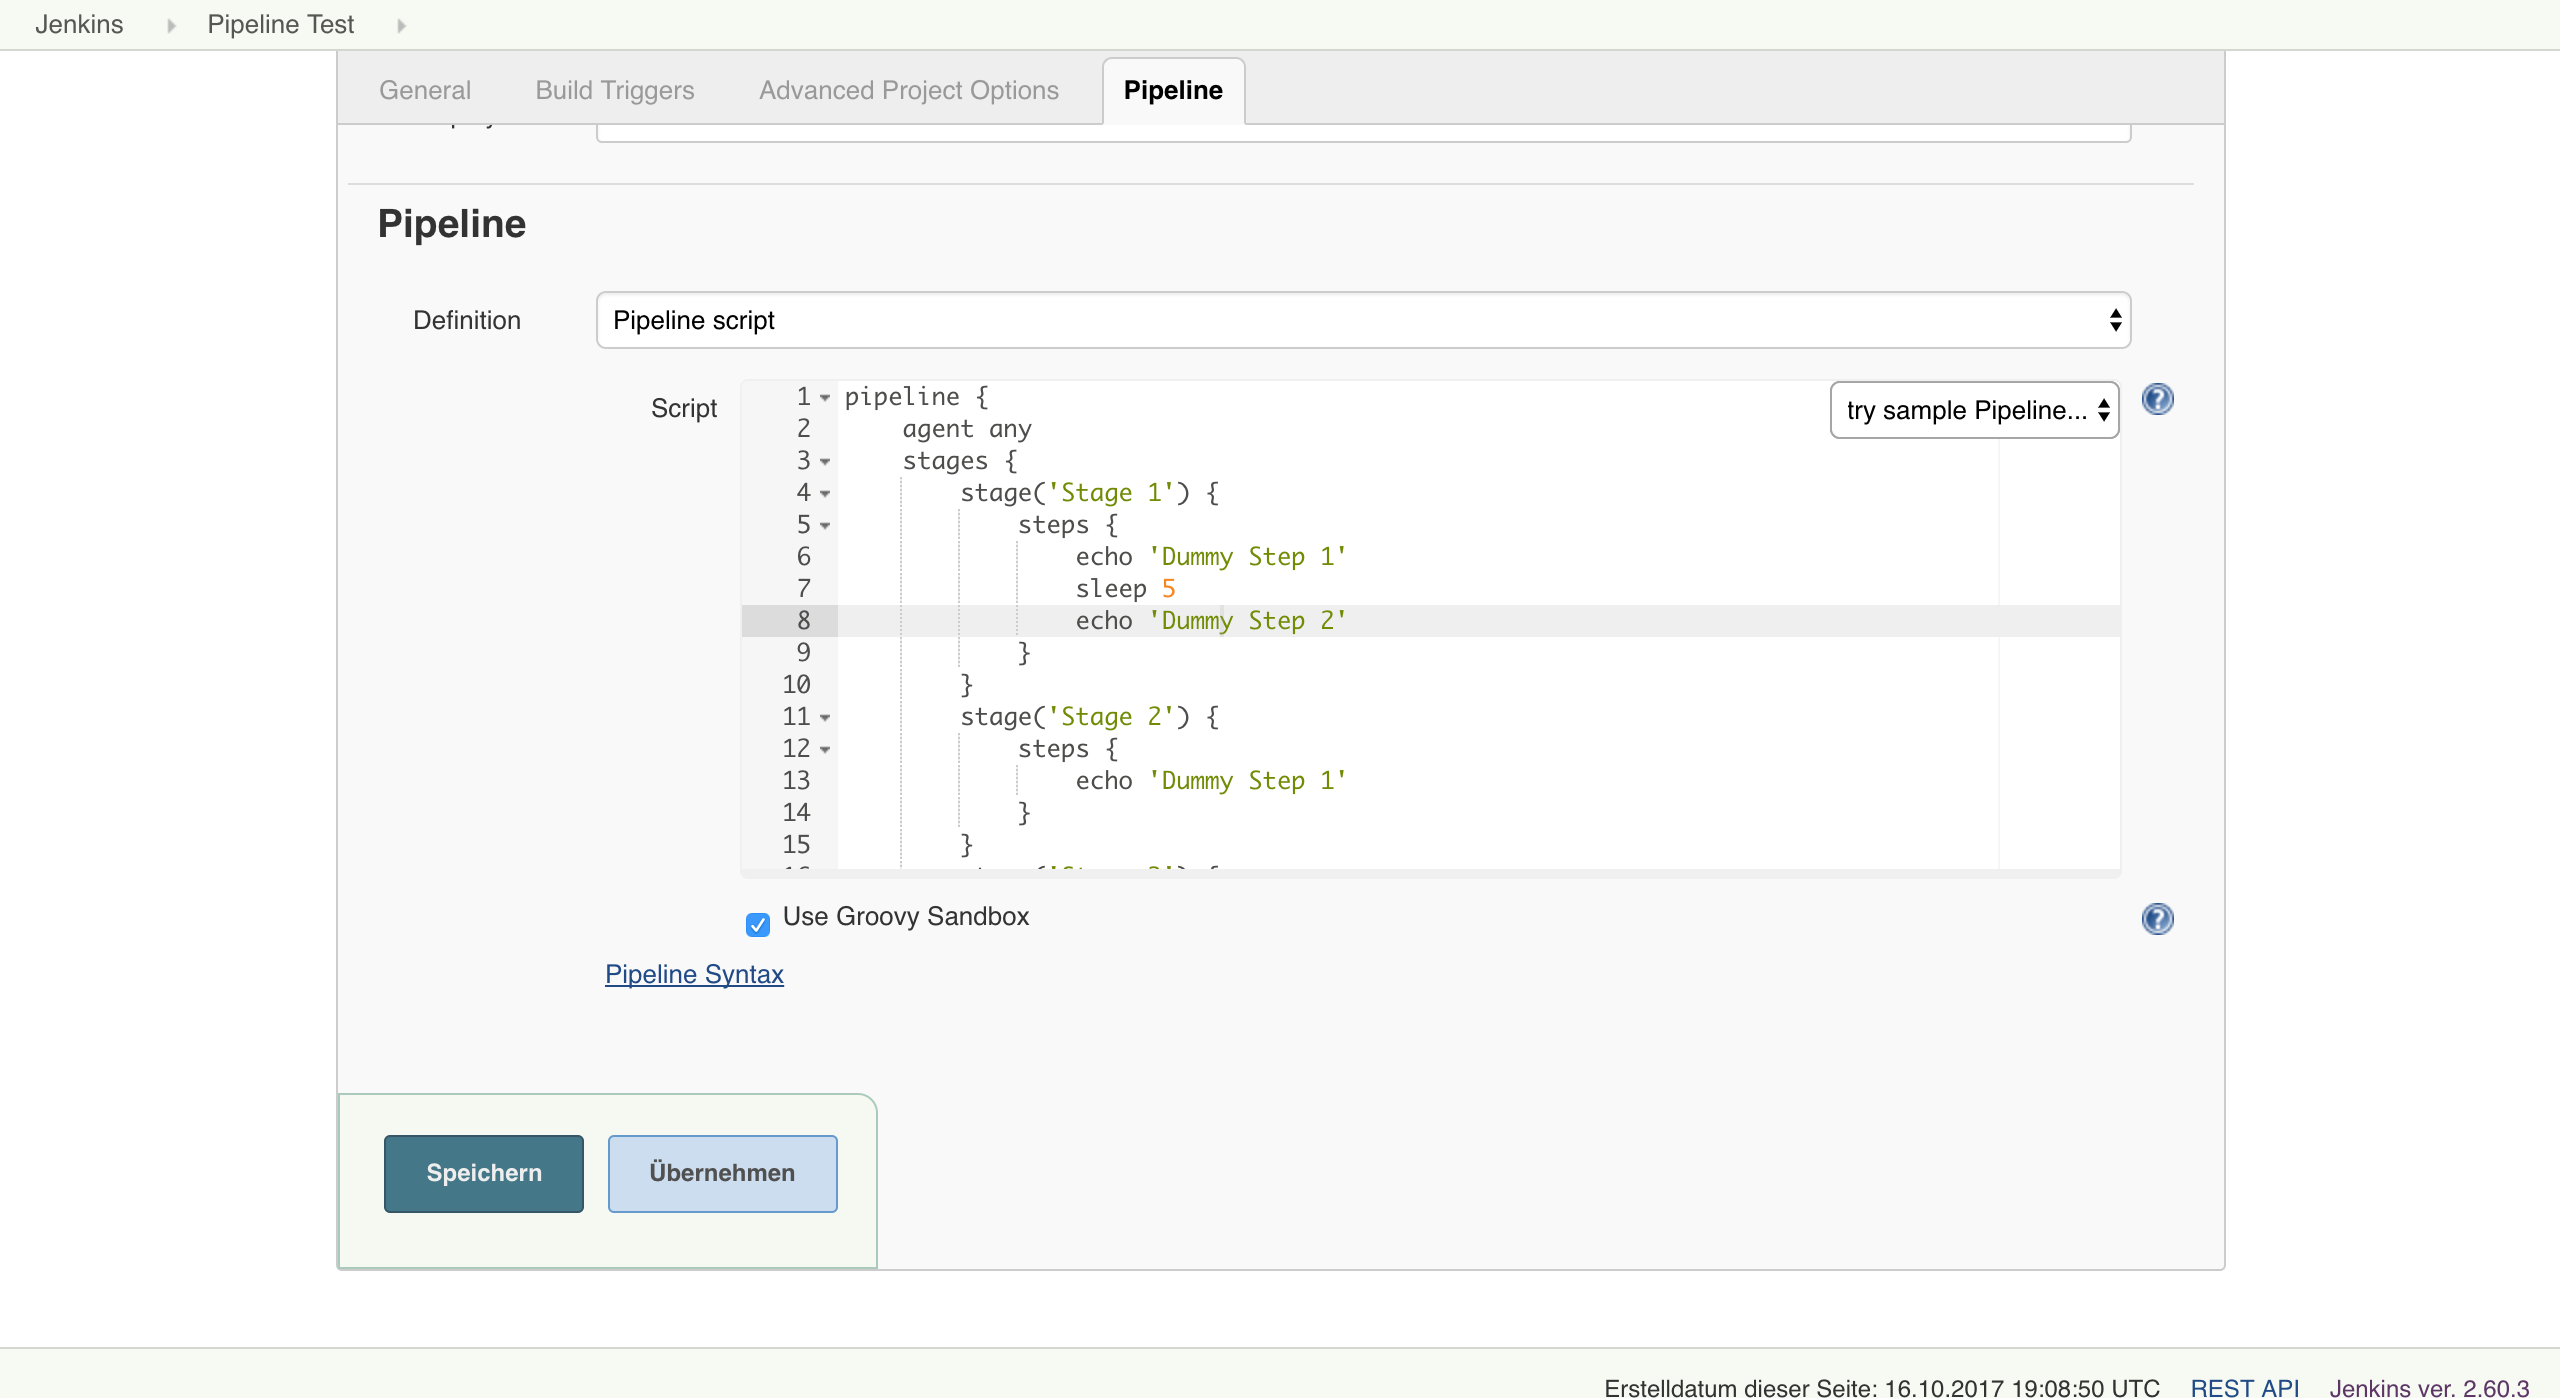
\includegraphics[width=.8\textwidth]{assets/jenkins-pipeline-script}
\end{figure}

Eine Pipeline wird bei Jenkins in der Skriptsprache Groovy geschrieben. Diese kann entweder über das Browser-Frontend oder über eine Konfigurationsdatei angelegt werden. In \figref{fig:jenkins-pipeline-config} wurde die Pipeline-Konfiguration über das Frontend angelegt. Vor der Pipeline-Konfiguration bietet Jenkins noch einige Einstellungsmöglichkeiten wie das deaktivieren von gleichzeitig laufenden Builds an.

\begin{figure}[h]
  \caption{Jenkins: Übersicht der Pipelines}
  \label{fig:jenkins-pipeline-overview}
  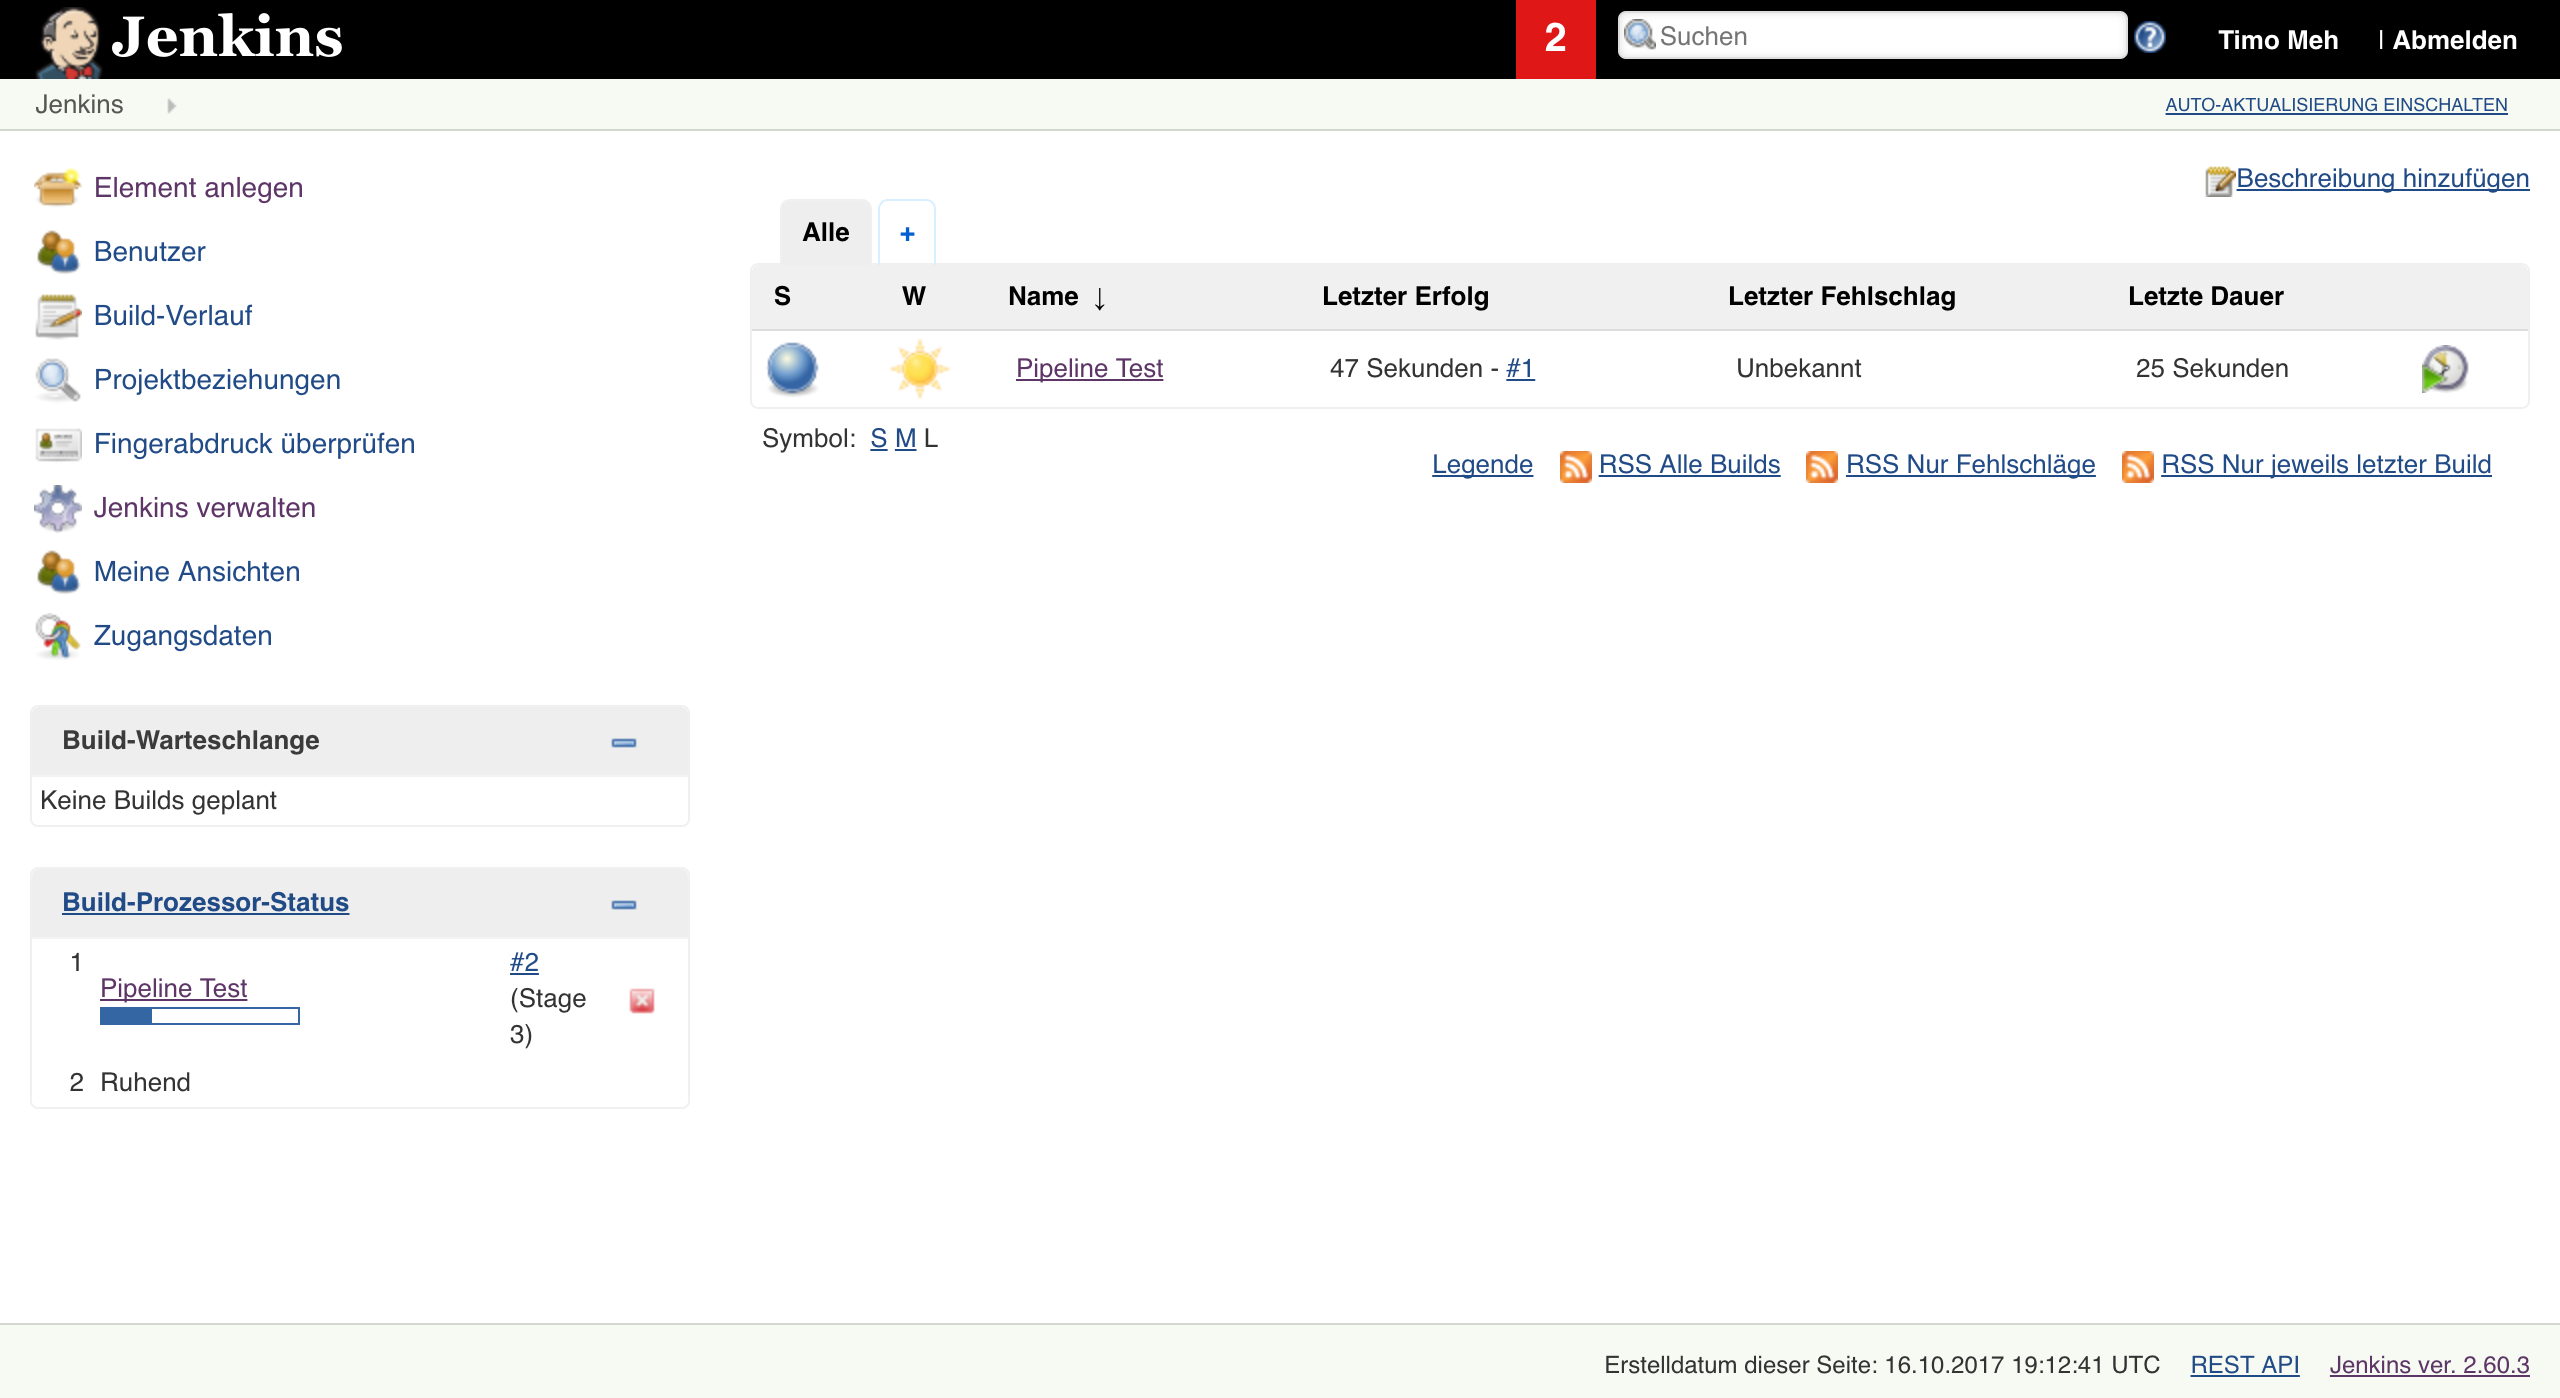
\includegraphics[width=.8\textwidth]{assets/jenkins-pipeline-overview}
\end{figure}

In der Übersicht (siehe \figref{fig:jenkins-pipeline-overview}) werden alle Pipelines mit Informationen zum letzten Build aufgelistet. Ein aktiver Build-Prozess wird seitlich unauffällig mit einem Ladebalken angezeigt.

\begin{figure}[h]
  \caption{Jenkins: Detailansicht eines aktiven Builds}
  \label{fig:jenkins-build-detail}
  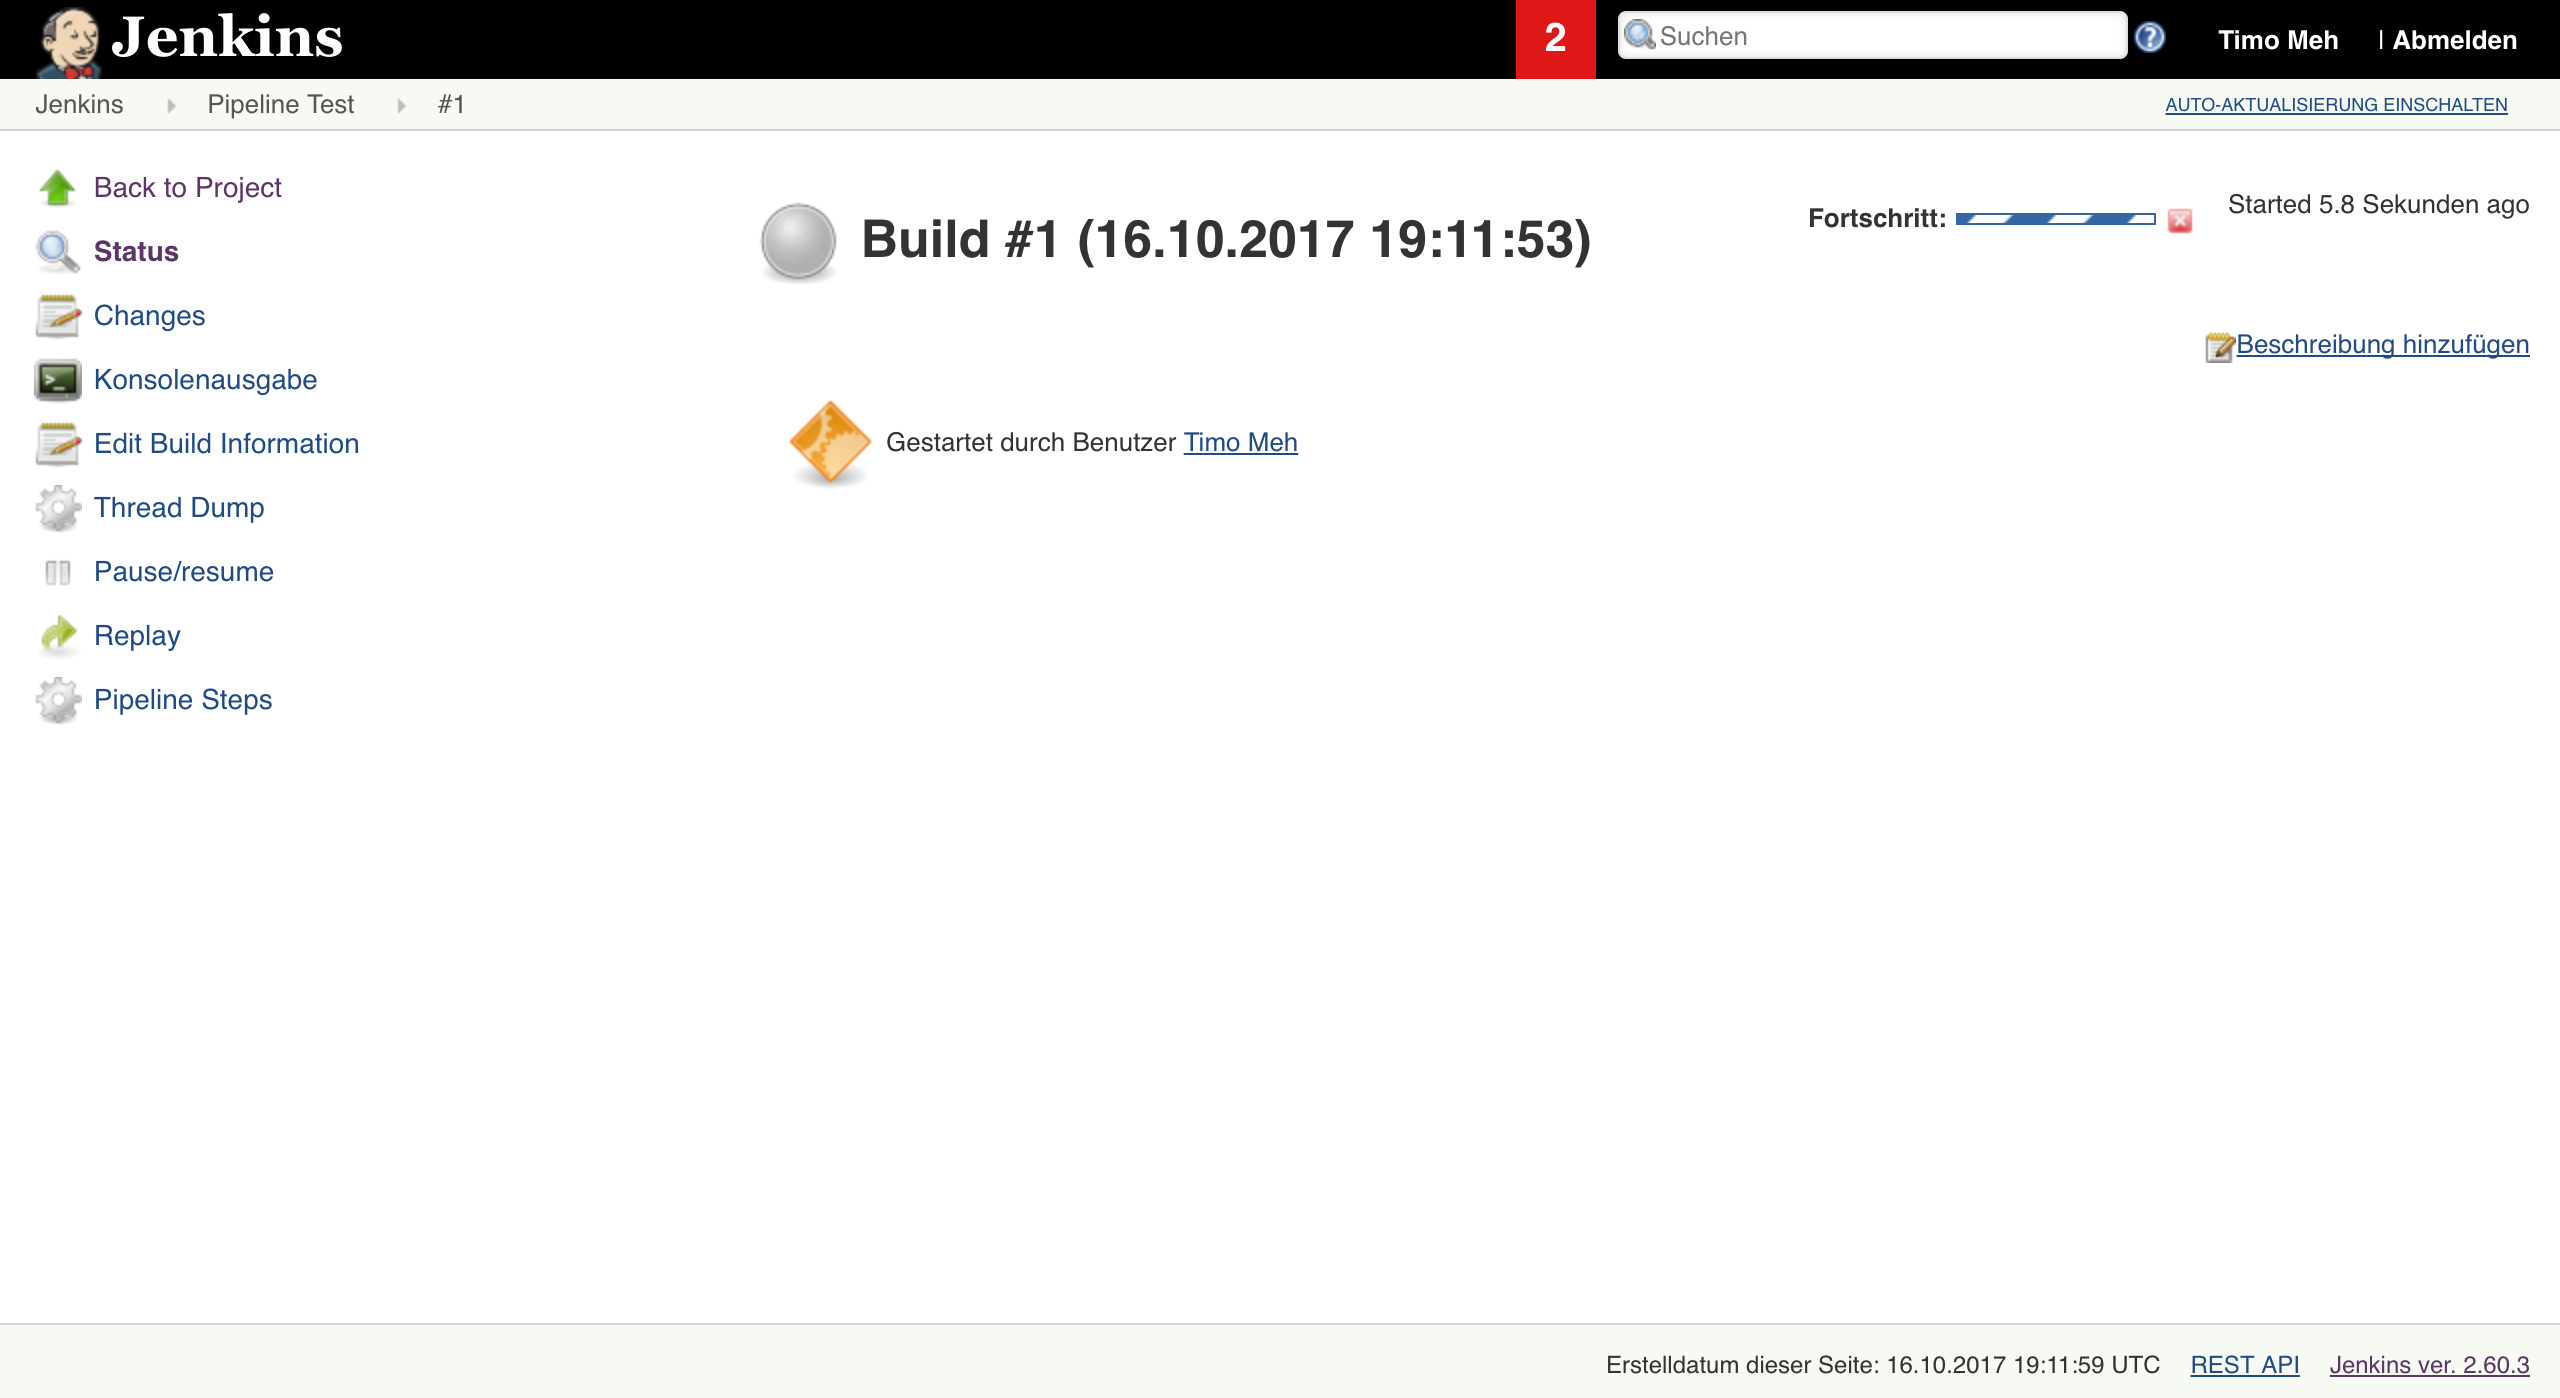
\includegraphics[width=.8\textwidth]{assets/jenkins-build-detail}
\end{figure}

Die Detailansicht eines Builds besitzt wenige Informationen (siehe \figref{fig:jenkins-build-detail}). Auf einer Unterseite wird die Konsolenausgabe der gesamten Pipeline angezeigt.

\subsection*{Vorteile von Jenkins}

\begin{itemize}
  \item Software ist kostenlos
  \item Seit vielen Jahren bewährt
  \item Große Community
  \item Lässt sich leicht auf vielen Umgebungen installieren
  \item Pipeline kann sowohl über den Browser als auch über eine Datei konfiguriert werden
  \item Pipeline kann beliebig strukturiert werden
  \item Builds können über einen \texttt{git push}, direkt, oder zeitgesteuert ausgeführt werden
\end{itemize}

\subsection*{Nachteile von Jenkins}

\begin{itemize}
  \item Muss selbst gehosted werden
  \item Nur so schnell wie die Maschine, auf der es läuft
  \item Keine Echtzeit-Updates im Browser
  \item Design ist in die Jahre gekommen und unübersichtlich
  \item Details zu einem Build-Prozess sind nicht direkt ersichtlich
  \item Da Groovy auf Java basiert, ist es abseits der Java-Welt weniger bekannt
\end{itemize}

\section{Travis CI}
\label{sec:analyse-travis}

Travis CI\footnote{https://travis-ci.com/ und https://travis-ci.org/}, im Folgenden verkürzt ``Travis'' genannt, ist ein Open Source Cloud-Dienst, dessen Fokus auf Continuous Integration liegt. Es lassen sich damit aber auch Deployments durchführen. Travis ist speziell für Repositories auf GitHub ausgelegt und unterstützt keine anderen Git-Remotes.

Für öffentliche Repositories ist Travis kostenlos, bei privaten Repositories fallen Kosten ab \$69 an. Mit ``Travis CI Enterprise'' besteht auch die Möglichkeit Travis selbst zu hosten. Abseits der Möglichkeit, privaten Repositories verwenden zu können, besitzt die kostenpflichtige Version nicht mehr Funktionalitäten als die kostenlose Version.

Durch die enge Integration an GitHub lässt sich Travis leicht zu einem Projekt hinzufügen: Mit einem Schalter lassen sich Build-Prozesse für ein Repository aktivieren (insofern man darauf Zugriff hat. Siehe \figref{fig:travis-activate}).

\begin{figure}[h]
  \caption{Travis CI: Aktivieren eines Build Prozess}
  \label{fig:travis-activate}
  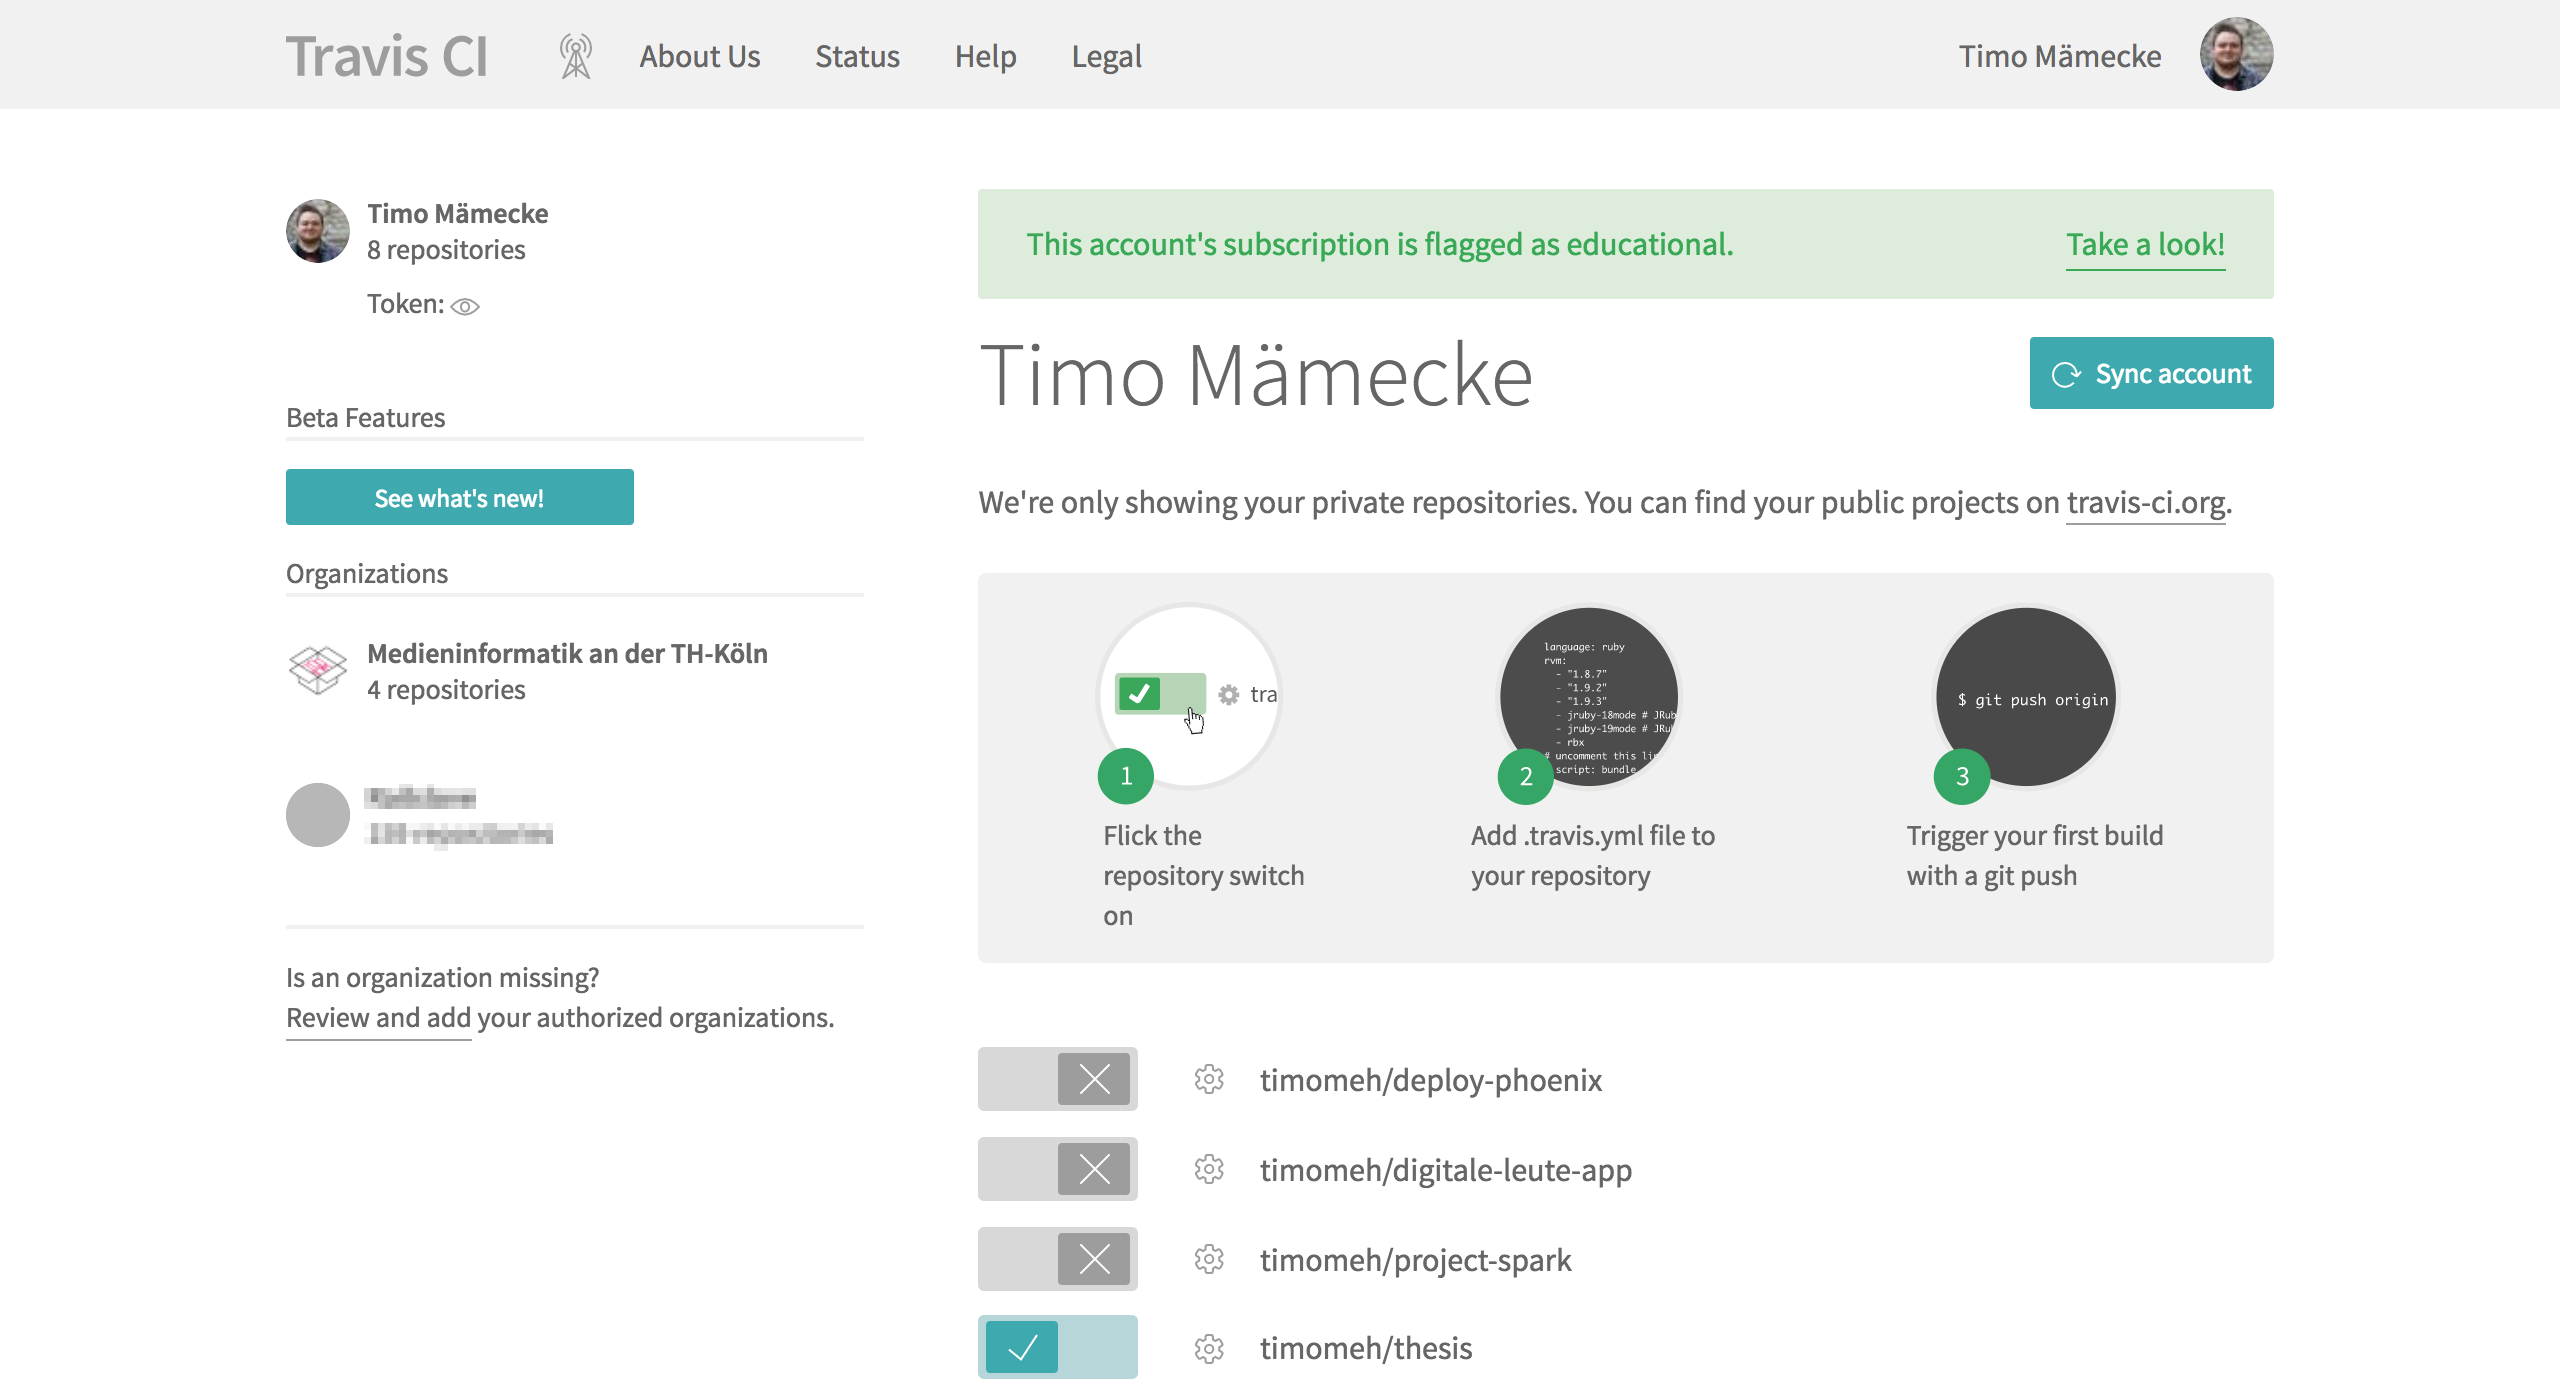
\includegraphics[width=.8\textwidth]{assets/travis-activate}
\end{figure}

Der Build-Prozess wird über die Datei \emph{.travis.yml} im Stammverzeichnis des Repositories konfiguriert. Mit Travis lassen sich jedoch keine Pipelines definieren, wie es bei Jenkins (\fullref{sec:analyse-jenkins}) der Fall ist. Travis besitzt vielmehr einen vorgefertigen Prozess, der über diese Datei genauer eingestellt werden kann.\footnote{vgl. https://docs.travis-ci.com/user/customizing-the-build/, abgerufen am 23.10.2017} Dadurch ist der Prozess zwar nicht so flexibel, jedoch kann dank solcher Standardeinstellungen die Konfiguration minimiert werden – bis zu einem Punkt, an dem überhaupt keine Konfiguration mehr notwendig ist.

Zum aktuellen Zeitpunkt wurden Stages als Beta-Funktionalität hinzugefügt.\footnote{vgl. https://docs.travis-ci.com/user/build-stages/, abgerufen am 23.10.2017} Damit lassen sich Schritte definieren, die einer Stage zugeordnet sind (siehe \lstref{lst:travis-config}).

\lstinputlisting
  [caption={Konfiguration eines Prozesses mit Travis CI Stages},
  label={lst:travis-config}]
  {snippets/travis-config-stages.yml}

Seitlich werden immer alle aktivierten Repositories, auf die man Zugriff hat, mit ihrem letzten Build-Status angezeigt (siehe \figref{fig:travis-running-build}). Der Fokus liegt also nicht auf den einzelnen Build-Prozessen, sondern dem Integrationsstatus des Repositories.

Im Hauptbereich der Ansicht sind jeweils Details zu einem Build-Prozess zu sehen. Bei der Verwendung von Stages werden die Schritte in ihrer Reihenfolge aufgelistet. Ohne Stages wird die Pipeline überhaupt nicht visualisiert, sondern die komplette Konsolenausgabe der Serverinstanz angezeigt.

\begin{figure}[h]
  \caption{Travis CI: Laufender Build-Prozess mit Stages}
  \label{fig:travis-running-build}
  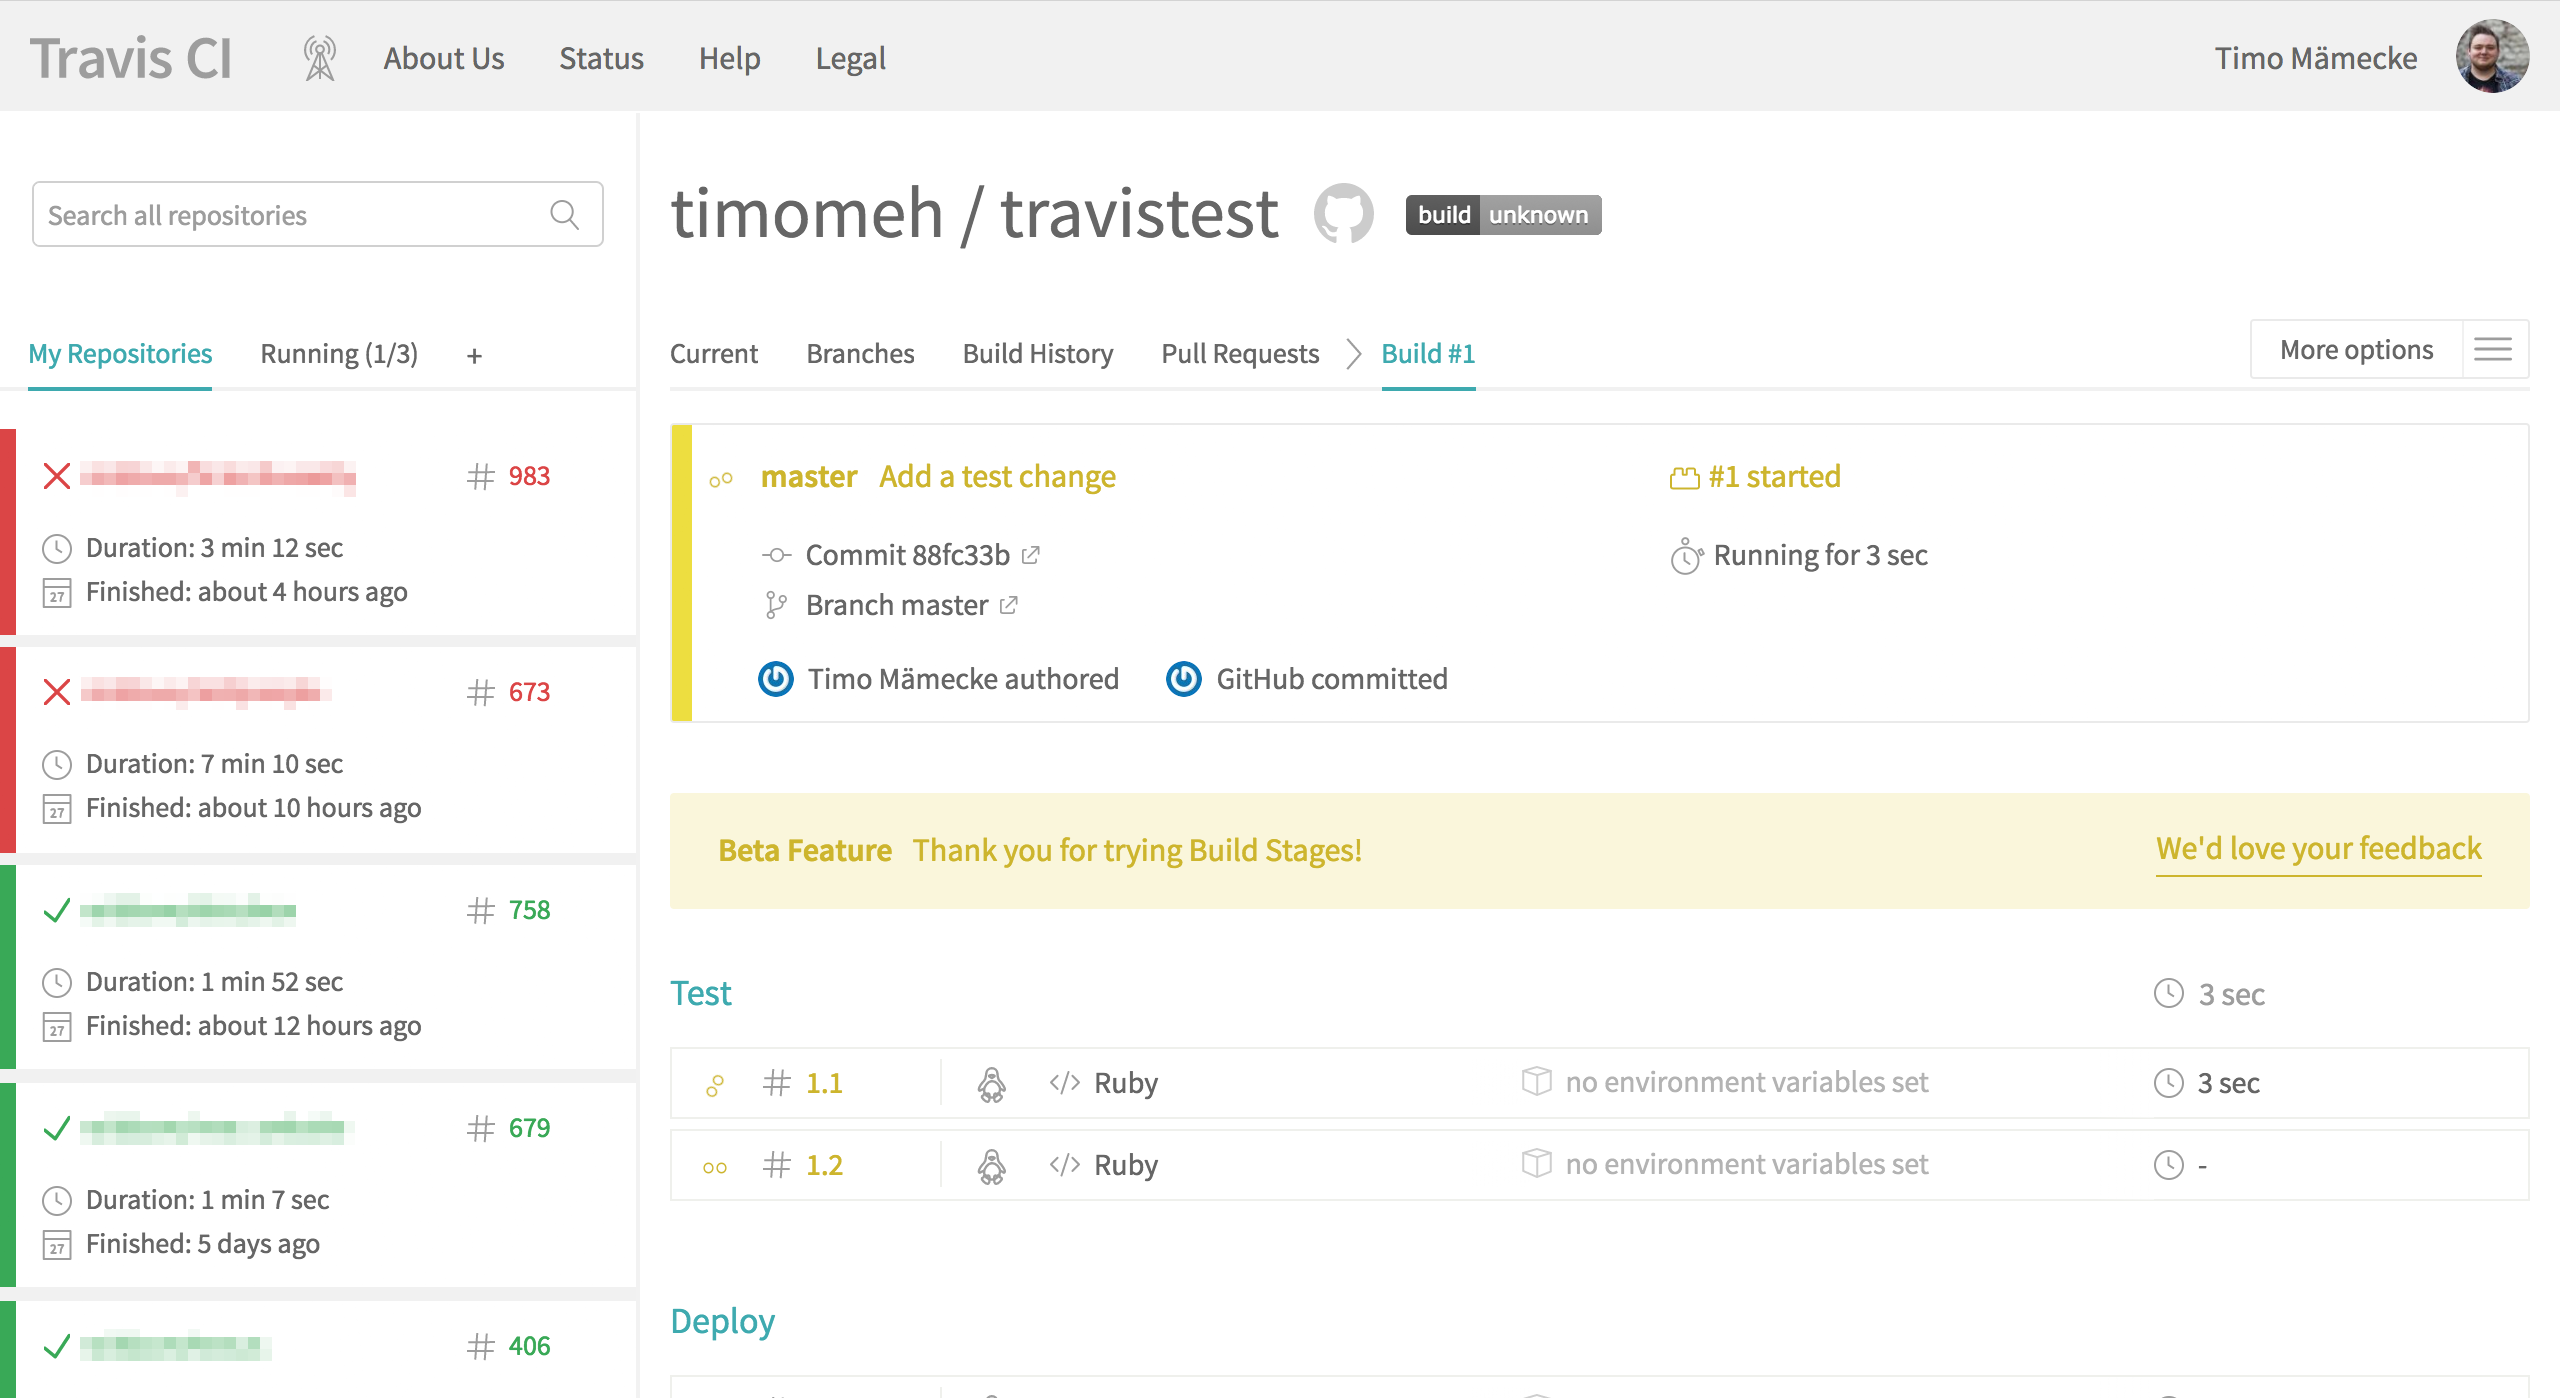
\includegraphics[width=.8\textwidth]{assets/travis-running-build}
\end{figure}

Travis zeigt viele hilfreiche Informationen wie Build-Zeiten und Daten aus Git an. Einige Informationen haben sich in Echtzeit aktualisiert, wobei andere Informationen erst nach erneutem Laden der Seite aktualisiert wurden.

Es gibt zudem eine komplette Historie der Build-Prozesse (siehe \figref{fig:travis-history}) und eine Übersicht der letzten Builds eines Branches (siehe \figref{fig:travis-branch}).

\begin{figure}[h]
  \caption{Travis CI: Build-Historie}
  \label{fig:travis-history}
  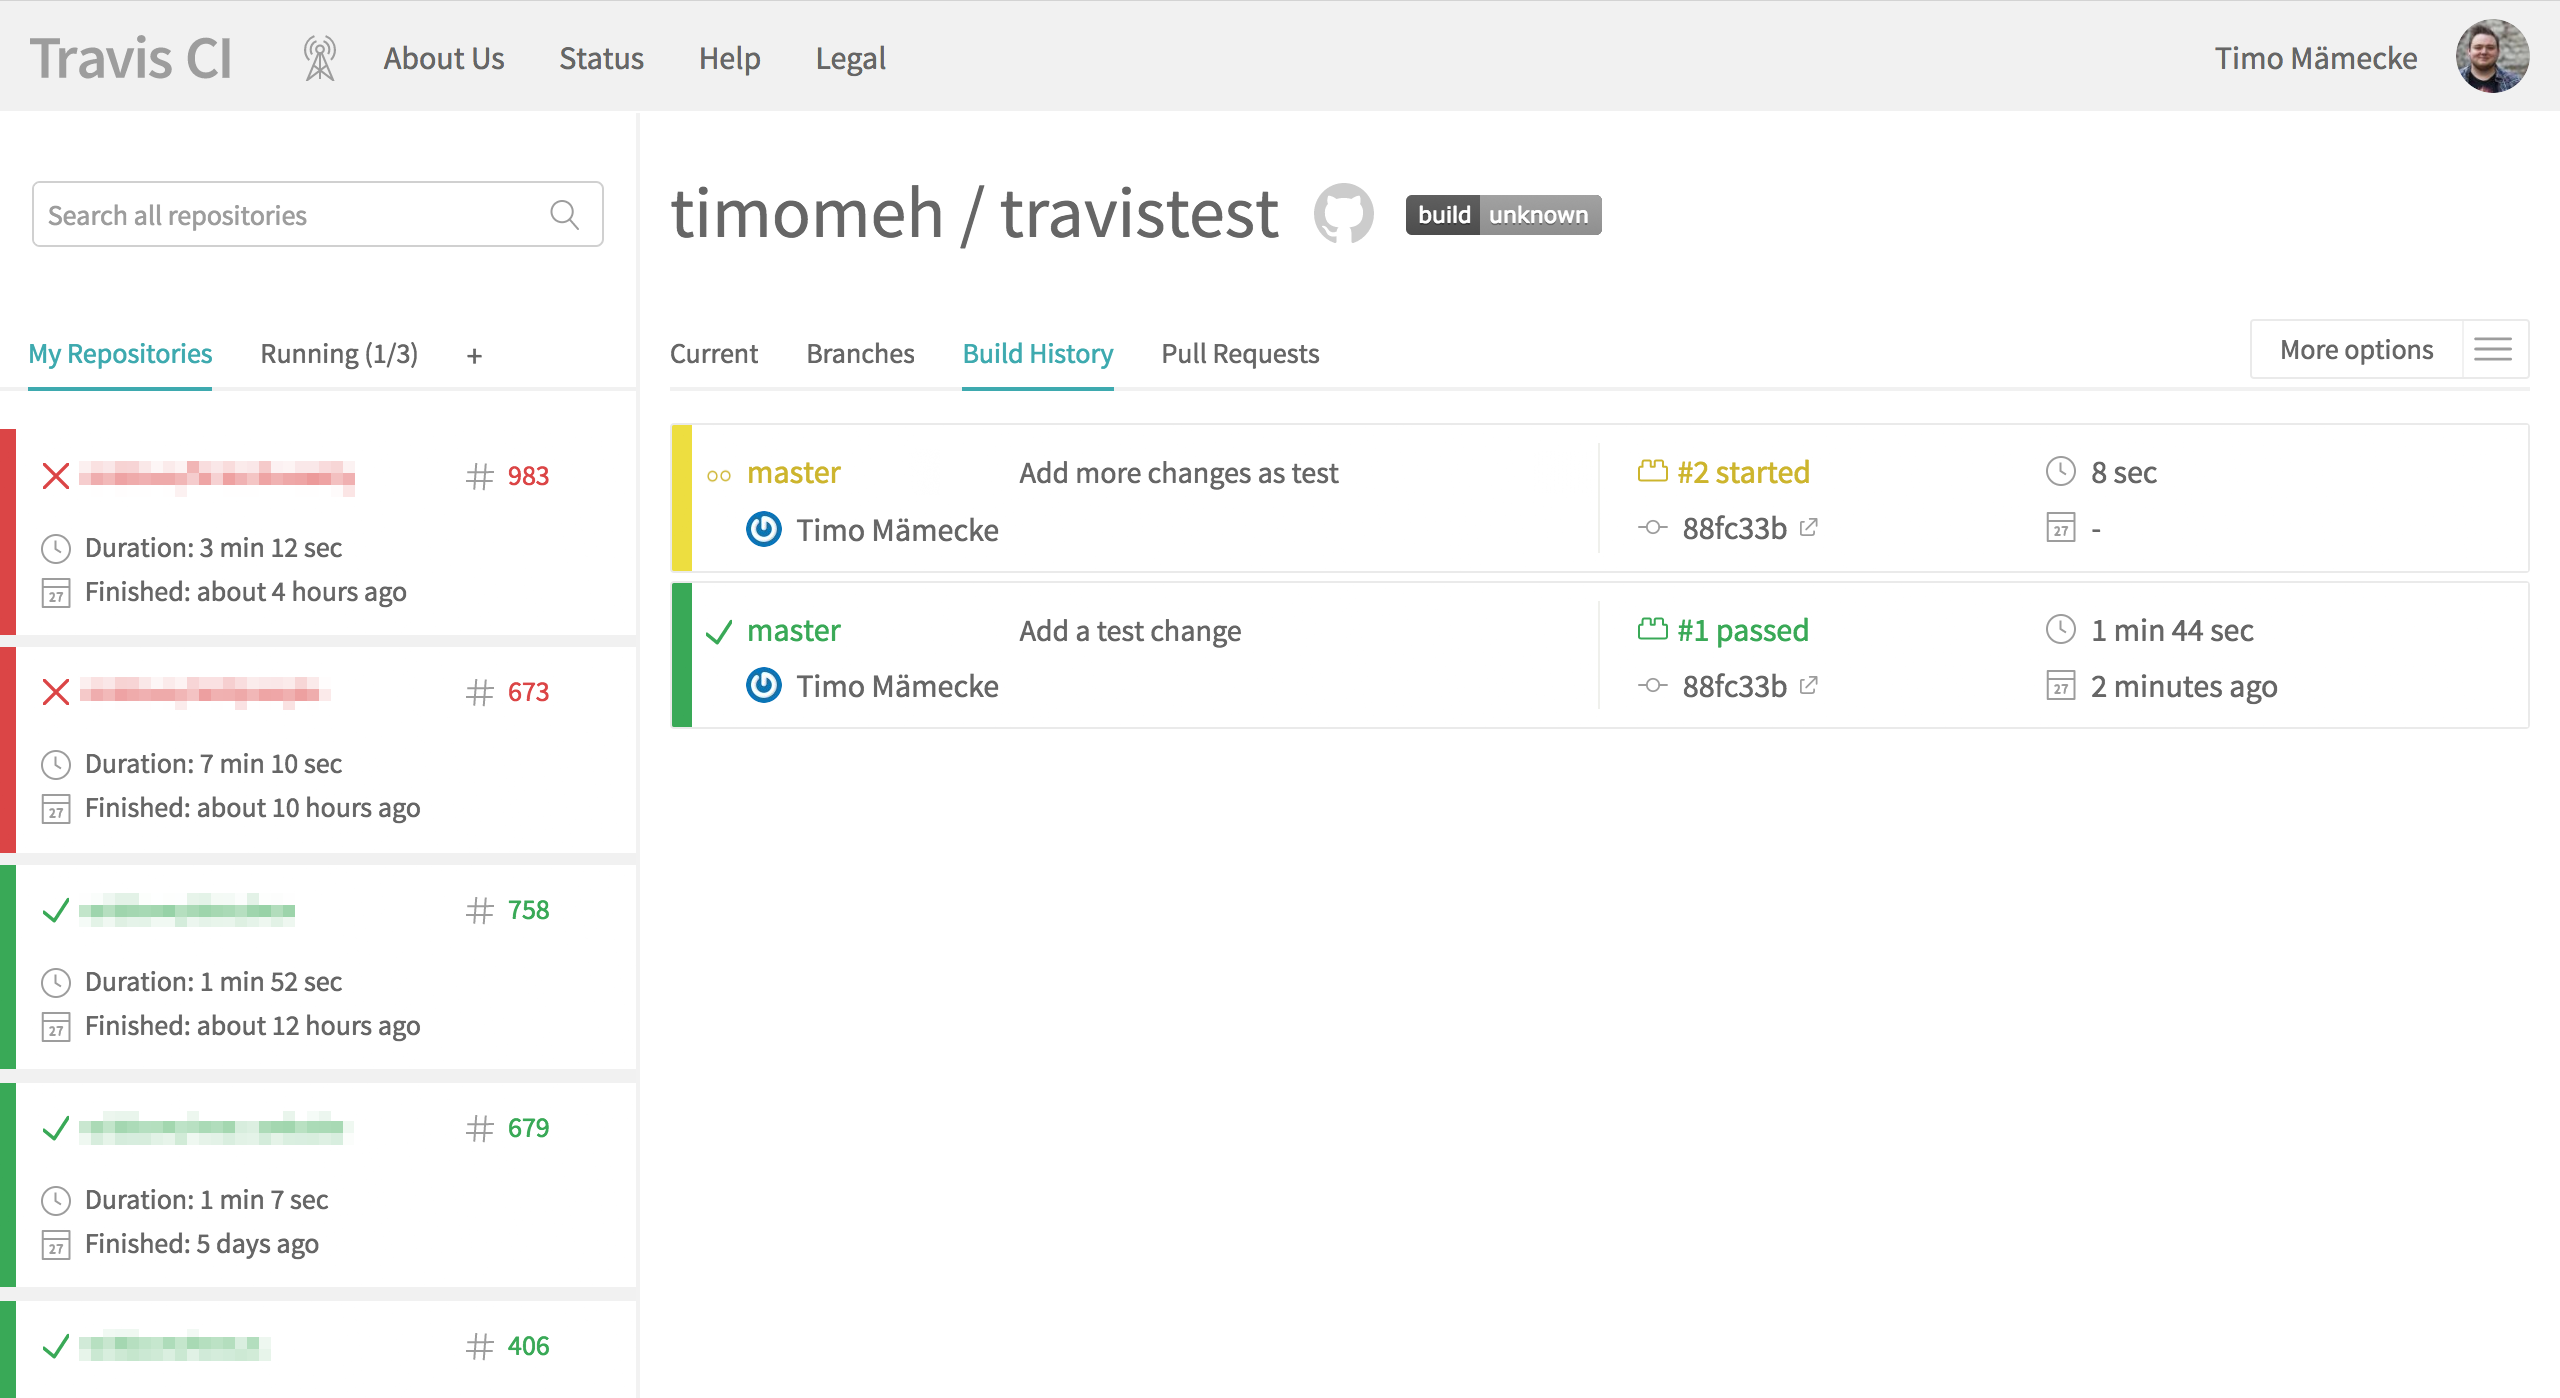
\includegraphics[width=.8\textwidth]{assets/travis-history}
\end{figure}

\begin{figure}[h]
  \caption{Travis CI: Übersicht nach Branches}
  \label{fig:travis-branch}
  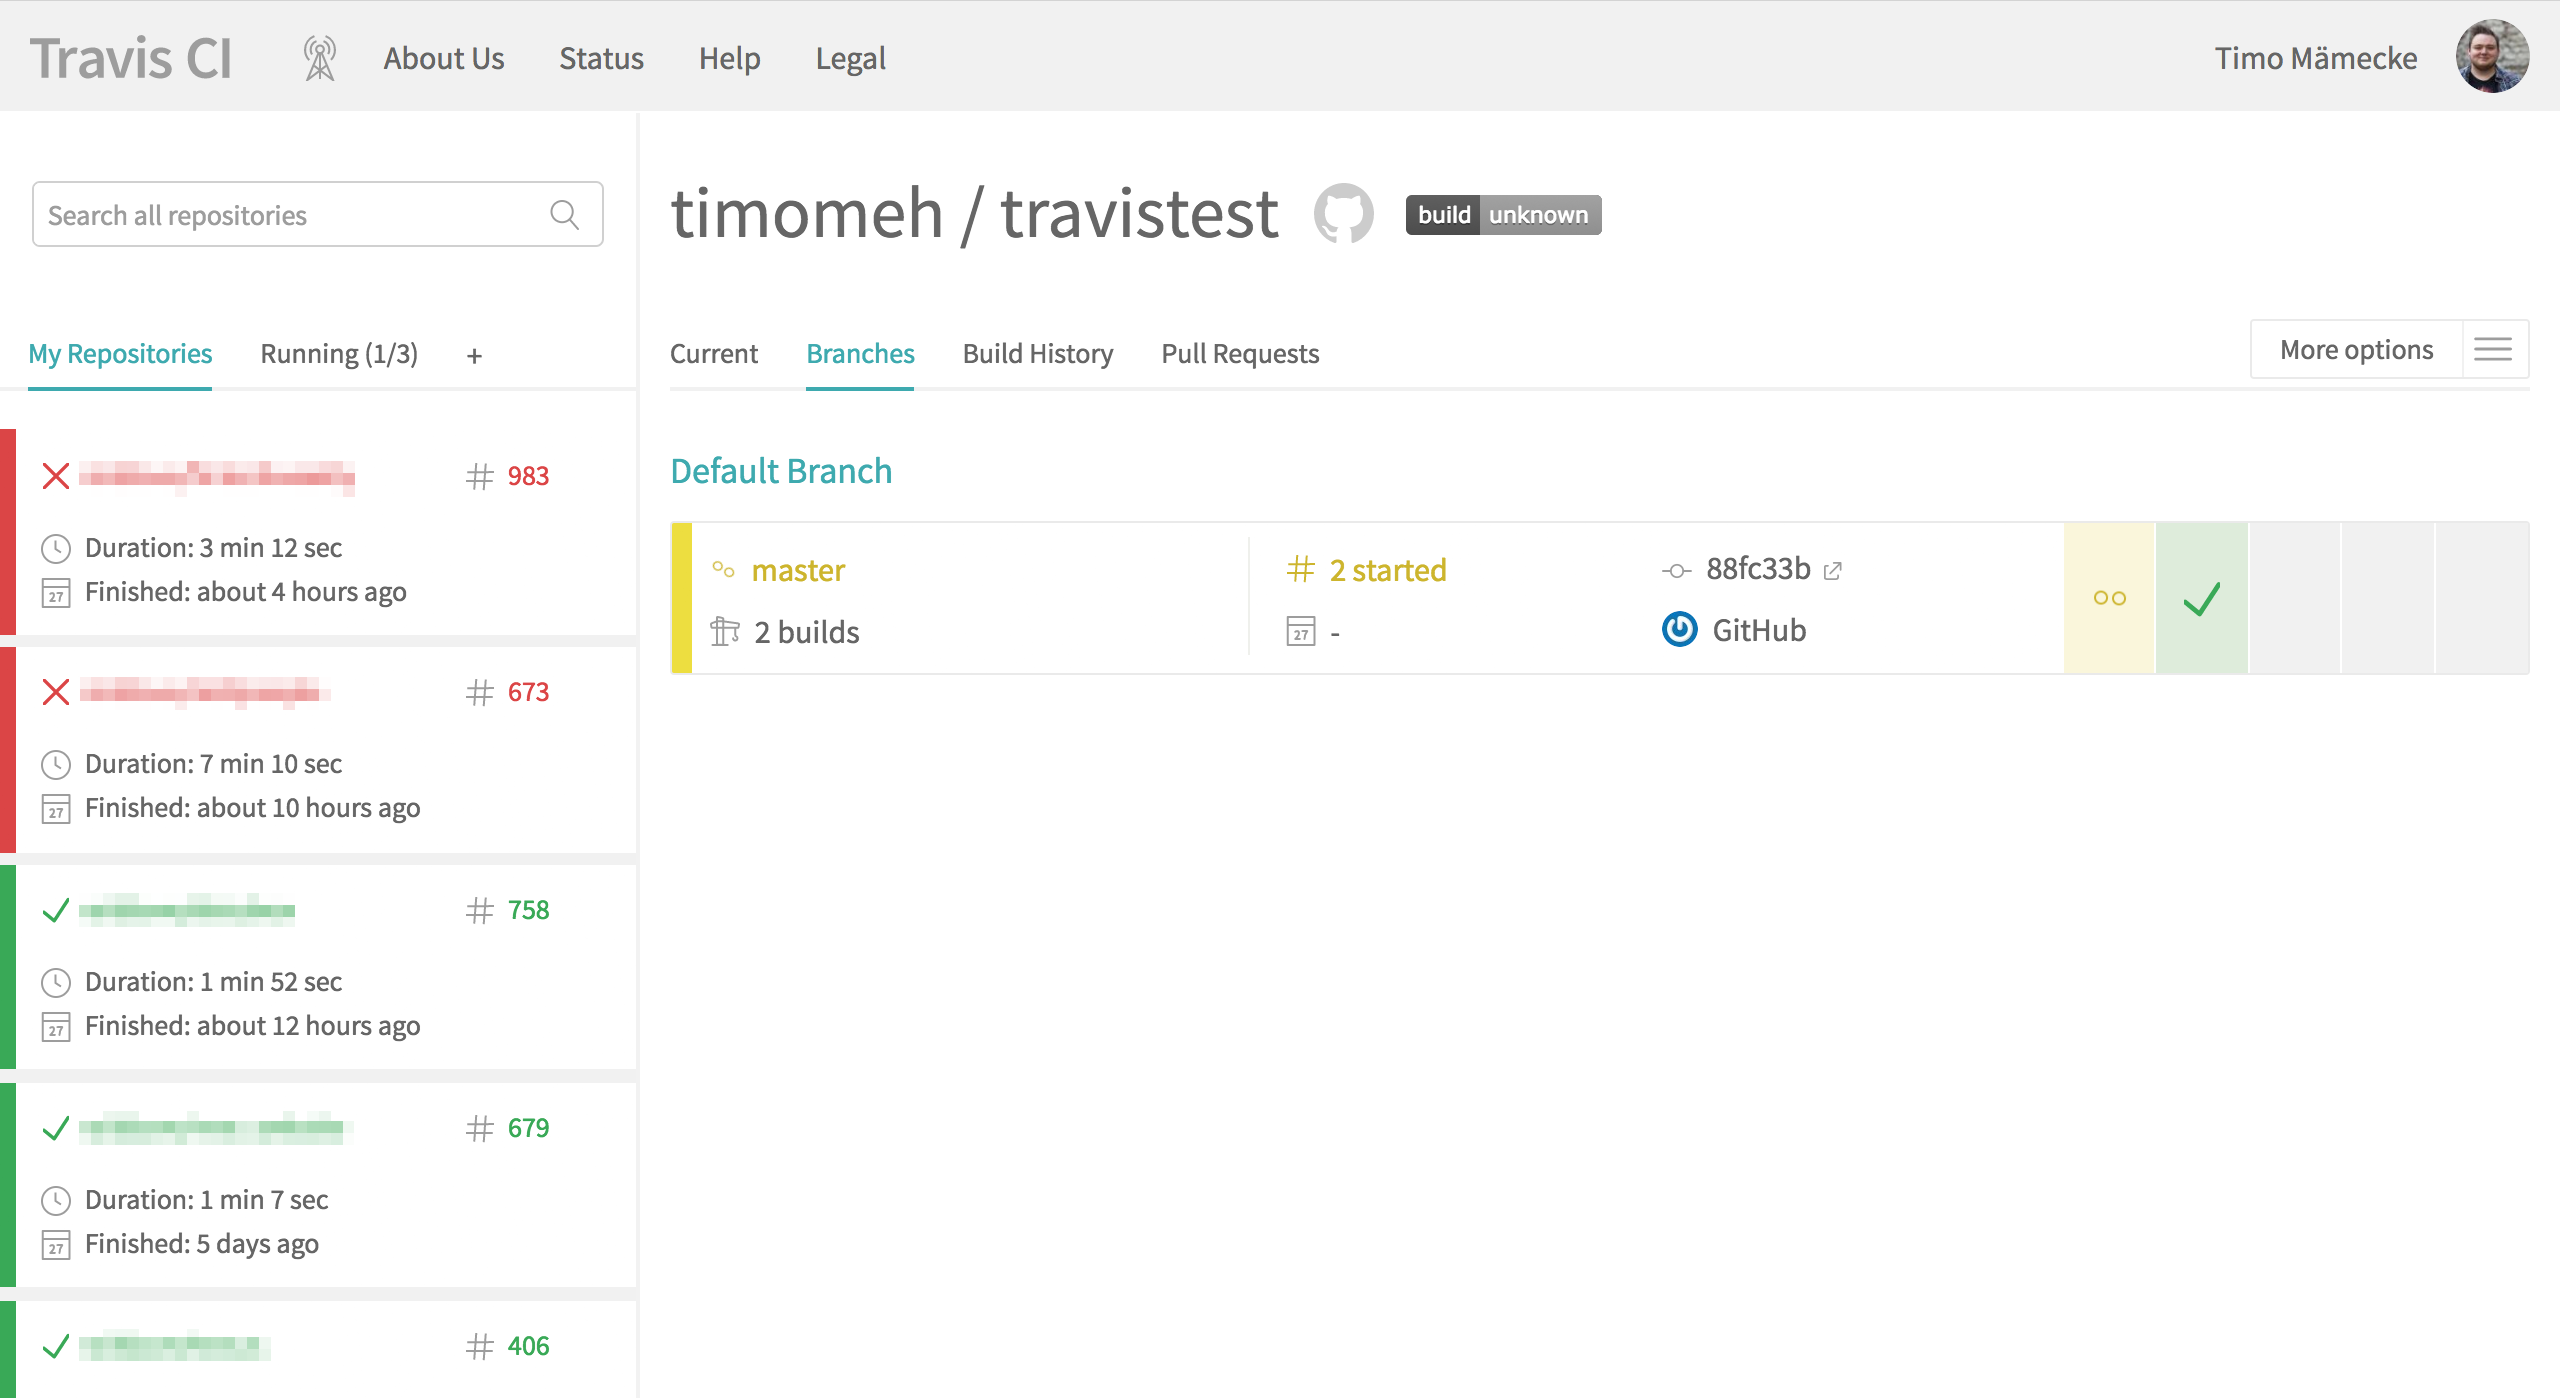
\includegraphics[width=.8\textwidth]{assets/travis-branch}
\end{figure}

Bei der Verwendung von Stages ist aufgefallen, dass Travis vor jedem Schritt zur Ausführung eine neue Instanz gestartet und initialisiert hat. Dieser Vorgang hat in einer Minimalkonfiguration bis zu 30 Sekunden gedauert, was sich sogar noch erhöhen kann, sobald externe Bibliotheken installiert werden müssen.

\subsection*{Vorteile von Travis CI}

\begin{itemize}
  \item Kostenlos für öffentliche Projekte
  \item Leicht integrierbar, kein großer Konfigurationsaufwand
  \item Modernes Design
  \item Klarer Fokus auf Continuous Integration
\end{itemize}

\subsection*{Nachteile von Travis CI}

\begin{itemize}
  \item Keine flexible Pipeline
  \item Keine Visualisierung der Pipeline
  \item Stages noch in Beta-Phase
  \item Es werden u.U. sehr viele Repositories angezeigt
  \item Funktioniert nur mit GitHub
  \item Builds können nicht zeitgesteuert gestartet werden
\end{itemize}

\section{Codeship}
\label{sec:analyse-codeship}

Codeship\footnote{https://codeship.com/} ist ein Cloud-Dienst, der sich in die zwei Modelle ``Codeship Basic'' und ``Codeship Pro'' aufteilt. Mit beiden lassen sich Pipelines definieren und ausführen. Codeship Basic kann kostenlos genutzt werden. Mehr Ressourcen und Funktionalitäten sind gegen Aufpreis ab \$49 verfügbar: beispielsweise lassen sich in der kostenlosen Version weder parallele Schritte ausführen noch Konfigurationsdateien nutzen.

Codeship Basic lässt sich über den Browser konfigurieren, Build-Prozesse werden in vorkonfigurierten Instanzen ausgeführt und Deployments können auf vorbestimmte Umgebungen durchgeführt werden. Im Vergleich dazu lässt sich Codeship in der Pro-Variante über Dateien konfigurieren, es können eigene Instanzen genutzt werden, und der gesamte Prozess inklusive Deployments ist anpassbar.

Codeship lässt sich mit Repositories in GitHub, Bitbucket und GitLab nutzen. Im Folgenden wurde die kostenlose Version von Codeship Basic genutzt.

Im Gegensatz zu Travis CI (siehe \fullref{sec:analyse-travis}) ist Codeship in Organisationen aufgeteilt. Jede Organisation besitzt daher eine eigene Übersicht.

Beim Einrichten über die Browser-Oberfläche stehen Formularfelder zur Verfügung (siehe \figref{fig:codeship-setup}), in die direkt Konfigurationen eingefügt werden, wie man es auch in einer Konfigurationsdatei tun würde.

\begin{figure}[h]
  \caption{Codeship: Einrichten eines Projekts}
  \label{fig:codeship-setup}
  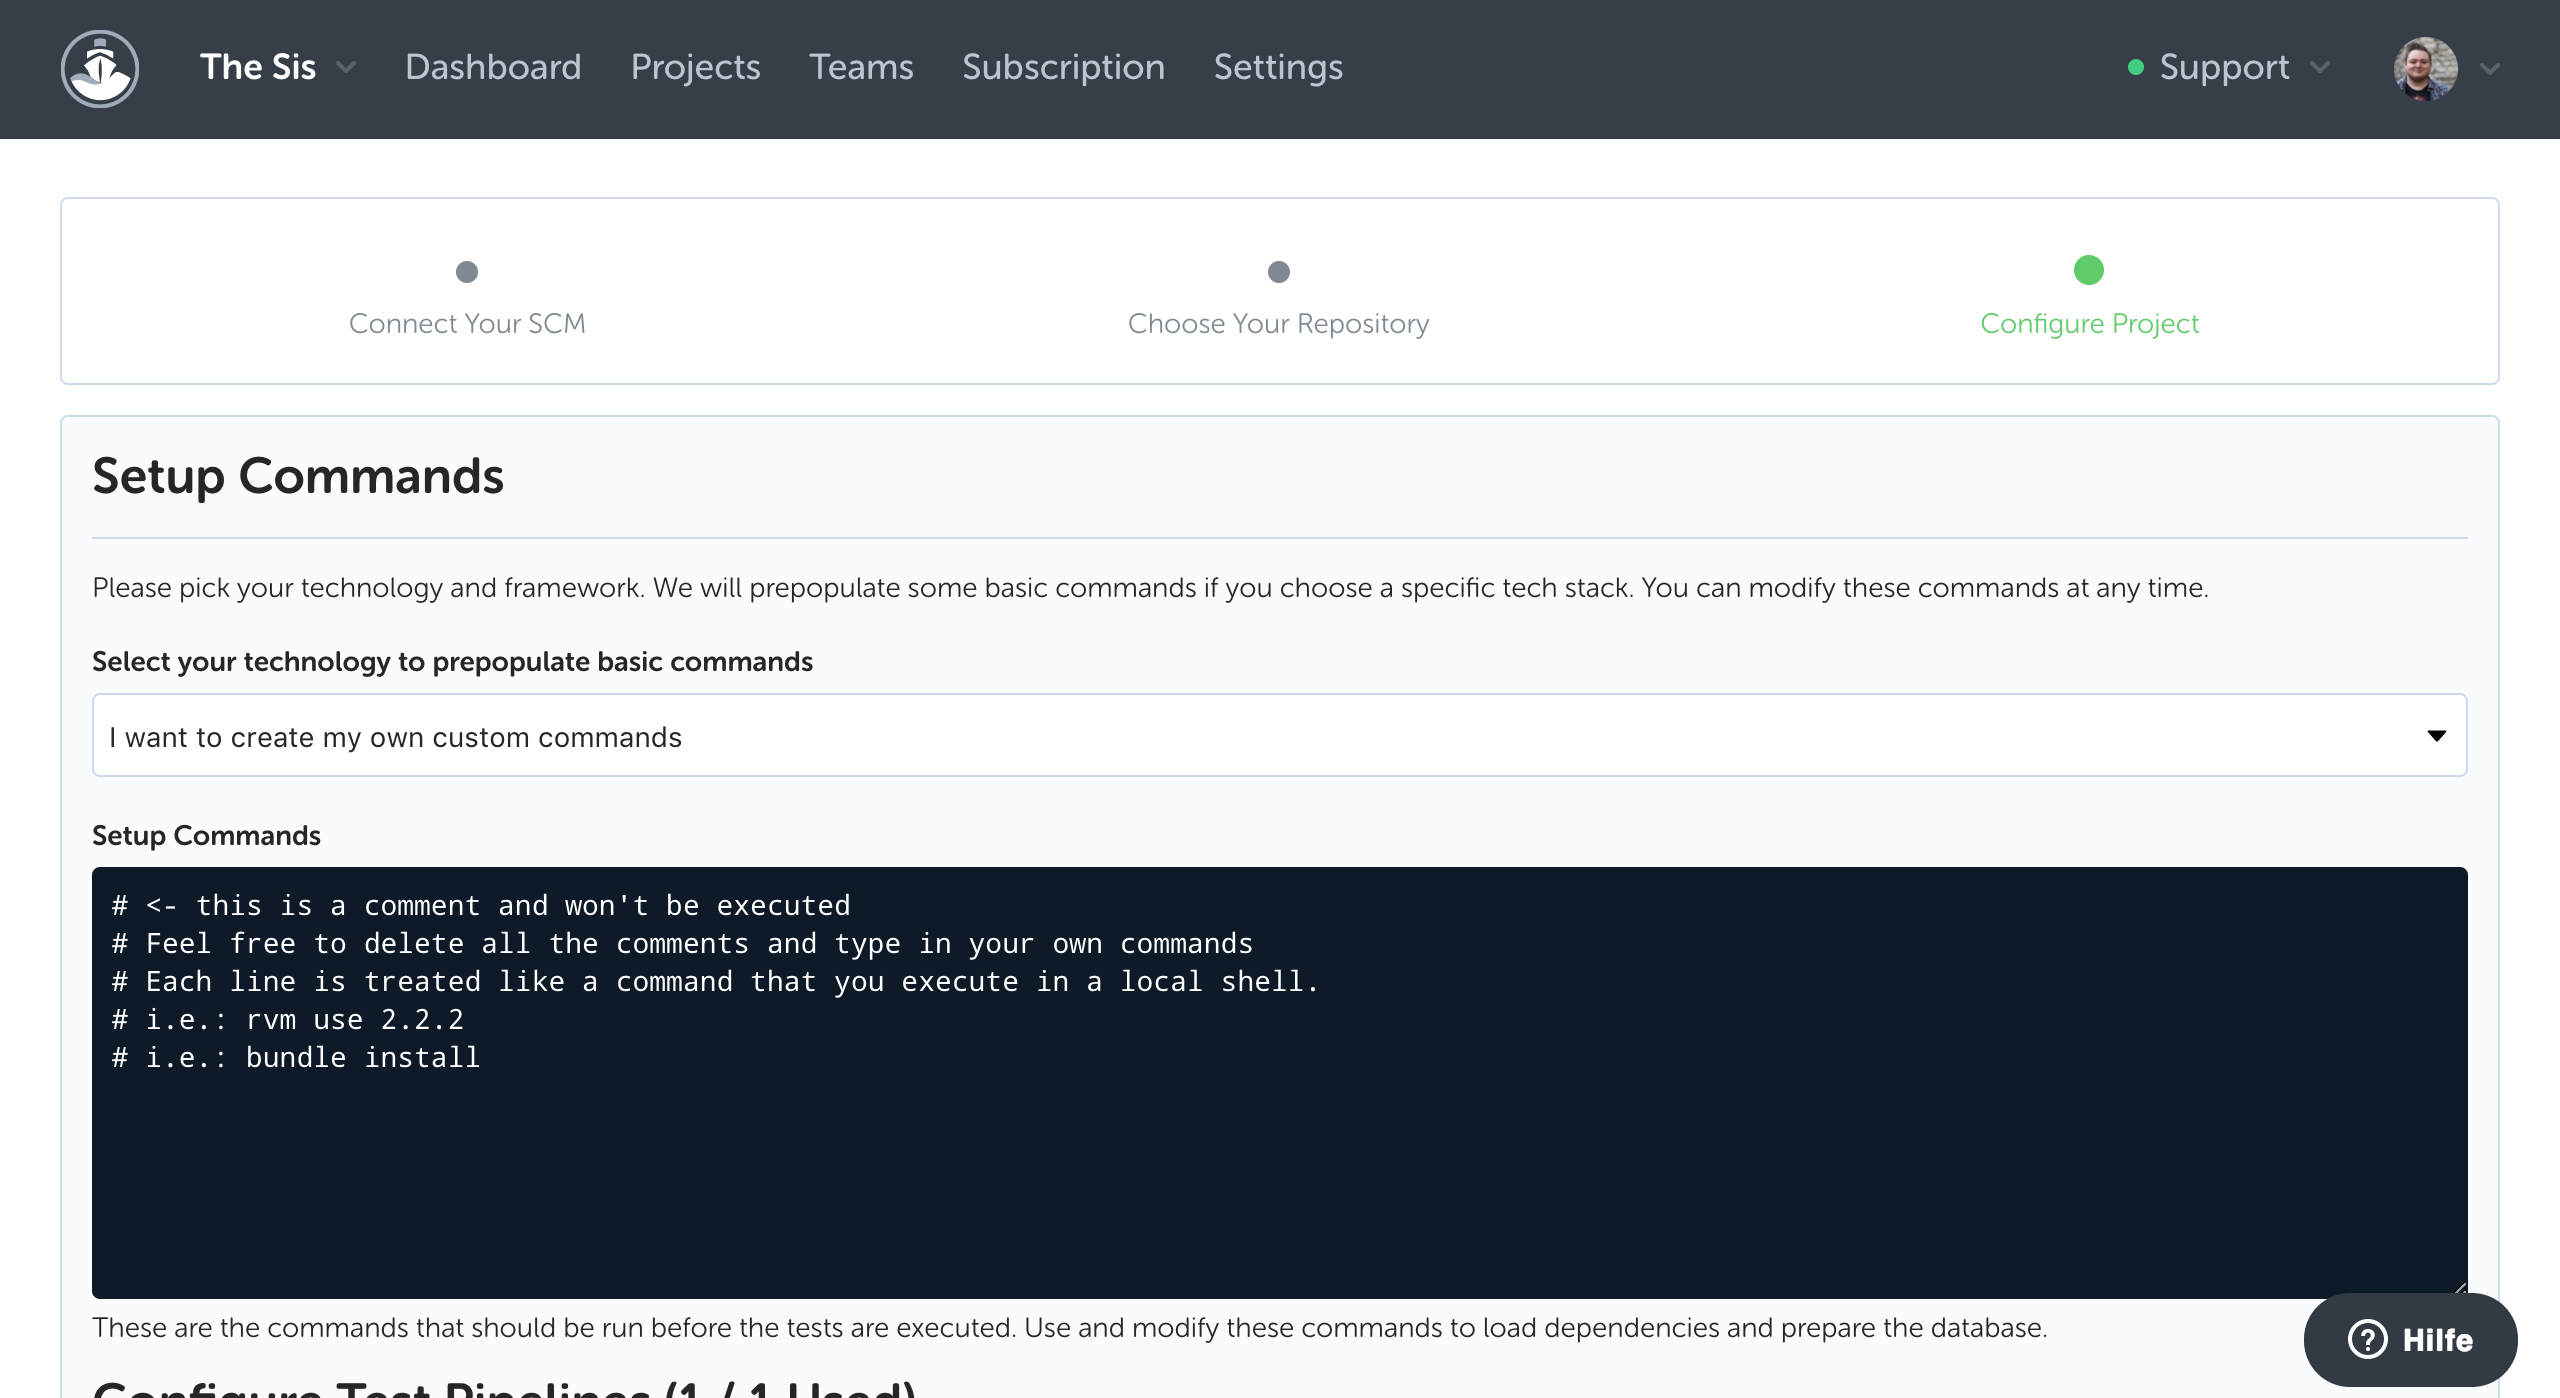
\includegraphics[width=.8\textwidth]{assets/codeship-setup}
\end{figure}

Es gibt (ähnlich zu Travis) eine Übersicht über alle Projekte inklusive ihrem letzten Status, eine chronologische Auflistung aller Builds (\figref{fig:codeship-builds}) und Informationen zu einem einzelnen Build (\figref{fig:codeship-build-details}).

\begin{figure}[h]
  \caption{Codeship: Auflistung aller Builds}
  \label{fig:codeship-builds}
  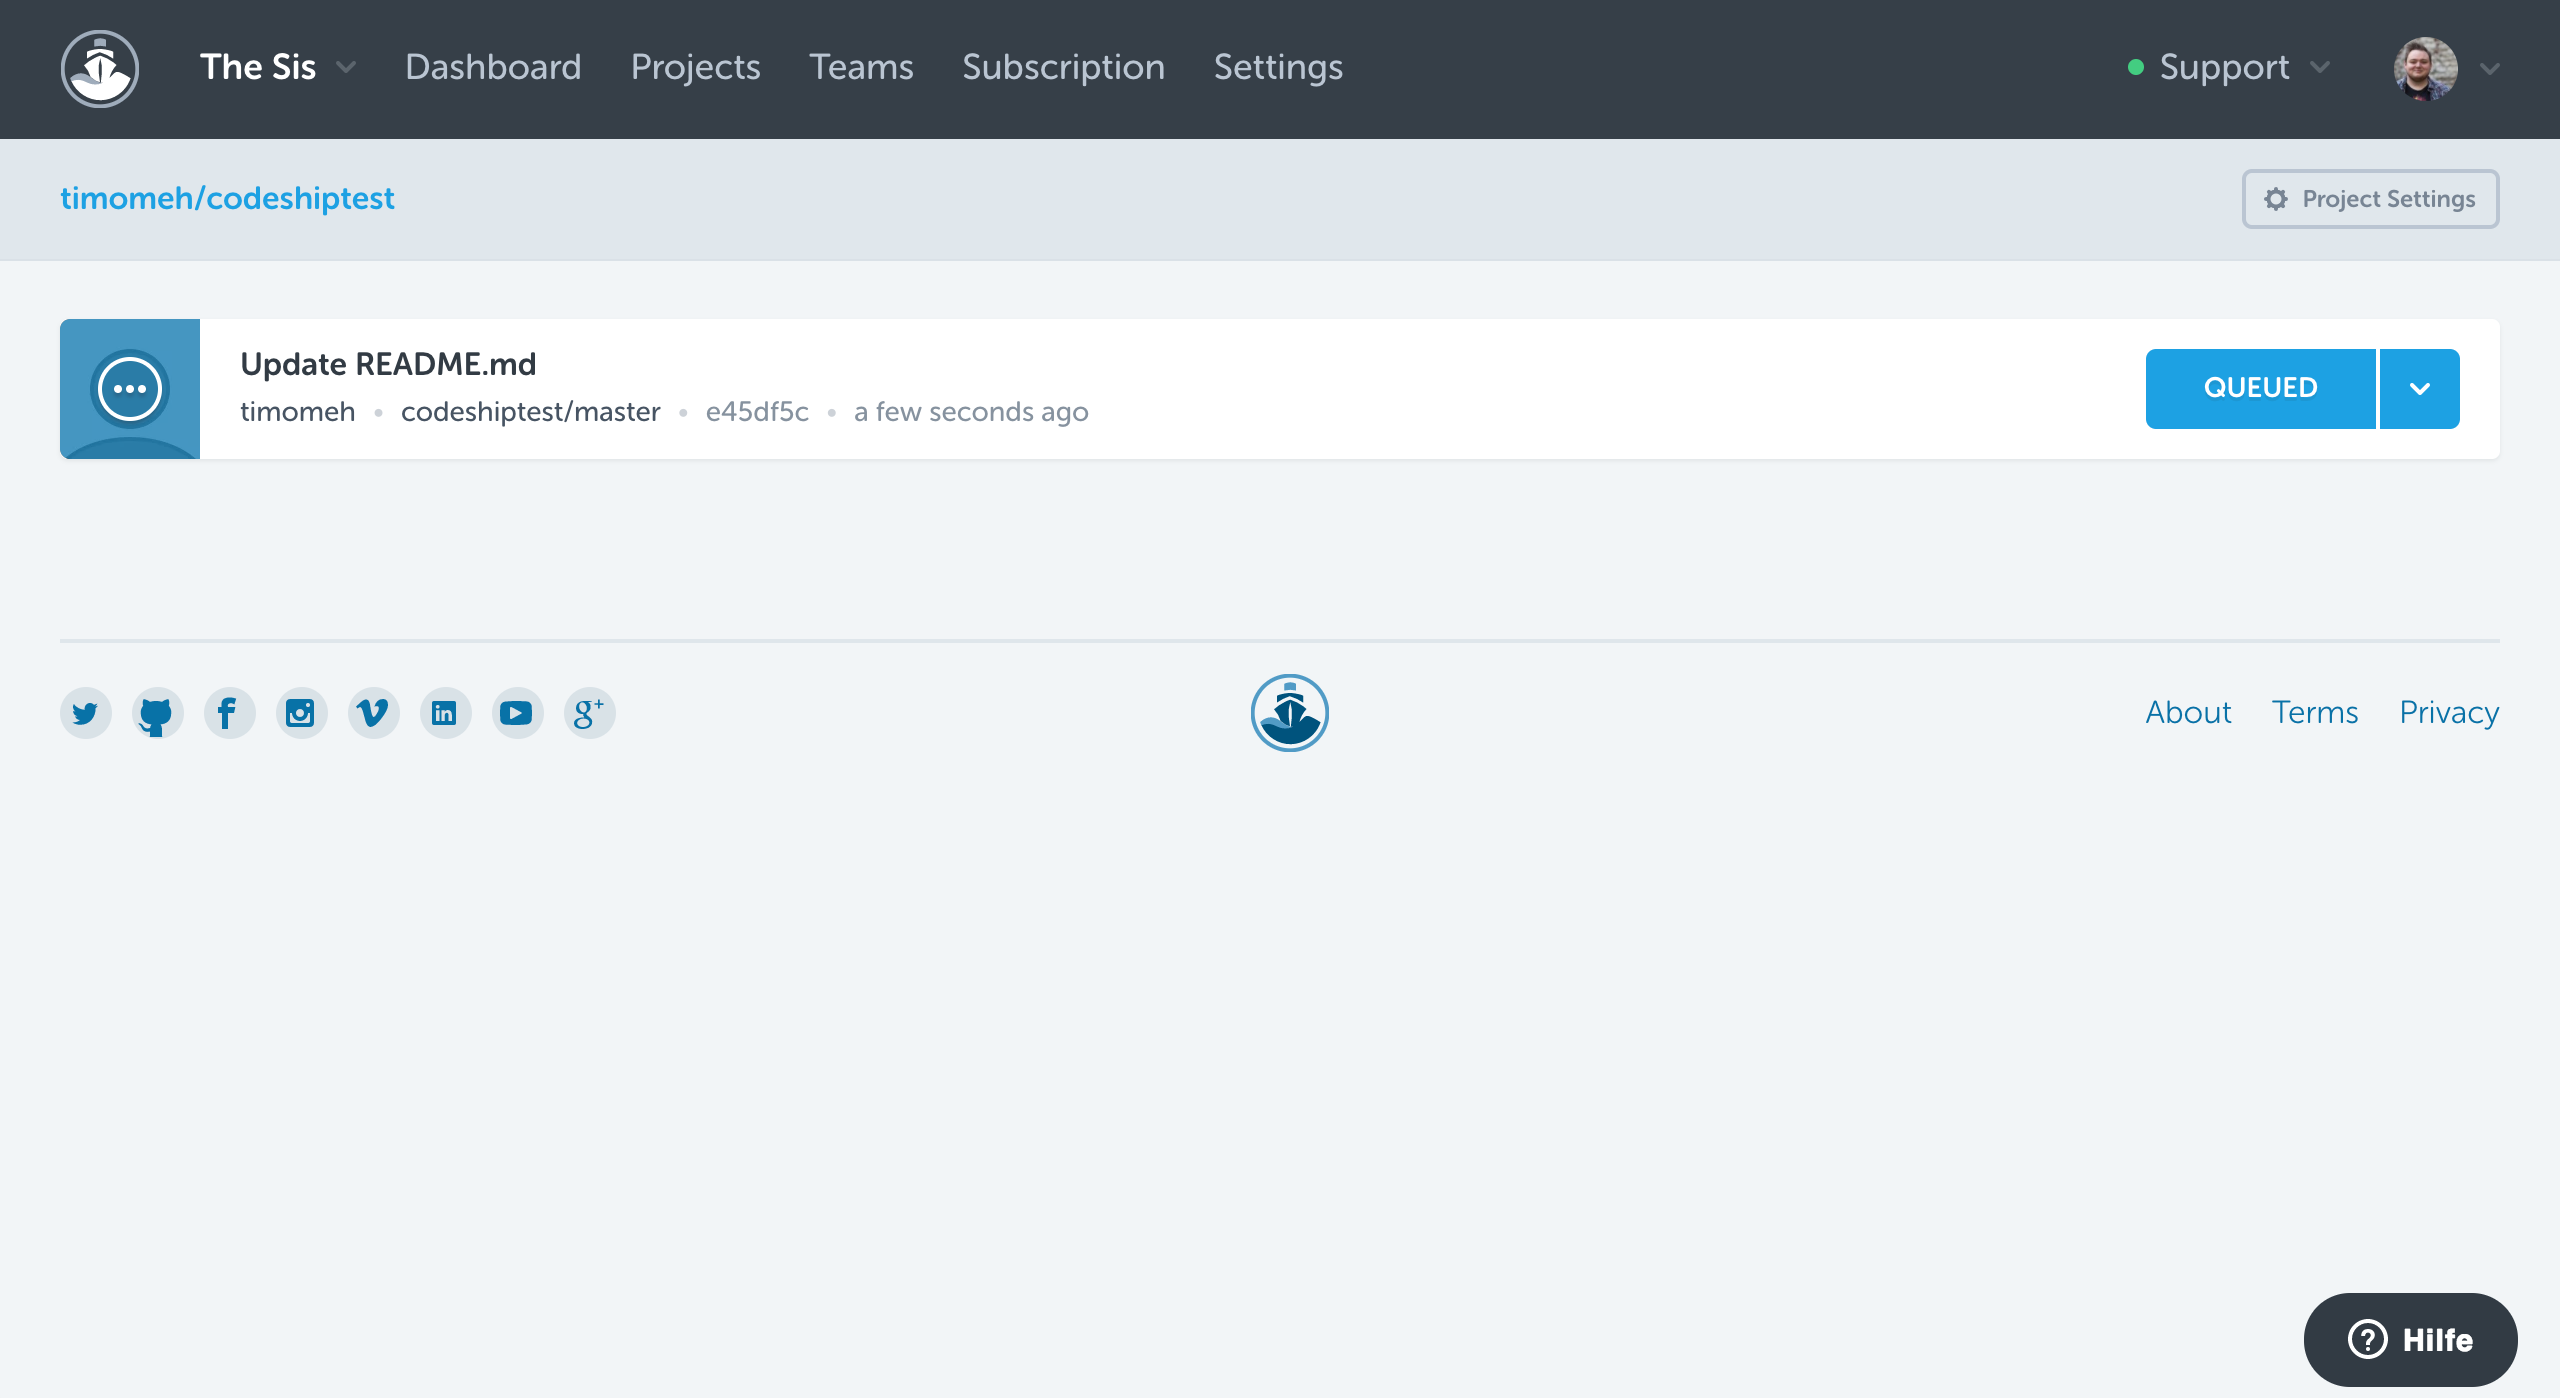
\includegraphics[width=.8\textwidth]{assets/codeship-builds}
\end{figure}

Im Gegensatz zu Travis CI visualisiert Codeship die gesamte Pipeline Schritt für Schritt und zeigt eine Konsolenausgabe je Schritt an.

\begin{figure}[h]
  \caption{Codeship: Ansicht eines Builds}
  \label{fig:codeship-build-details}
  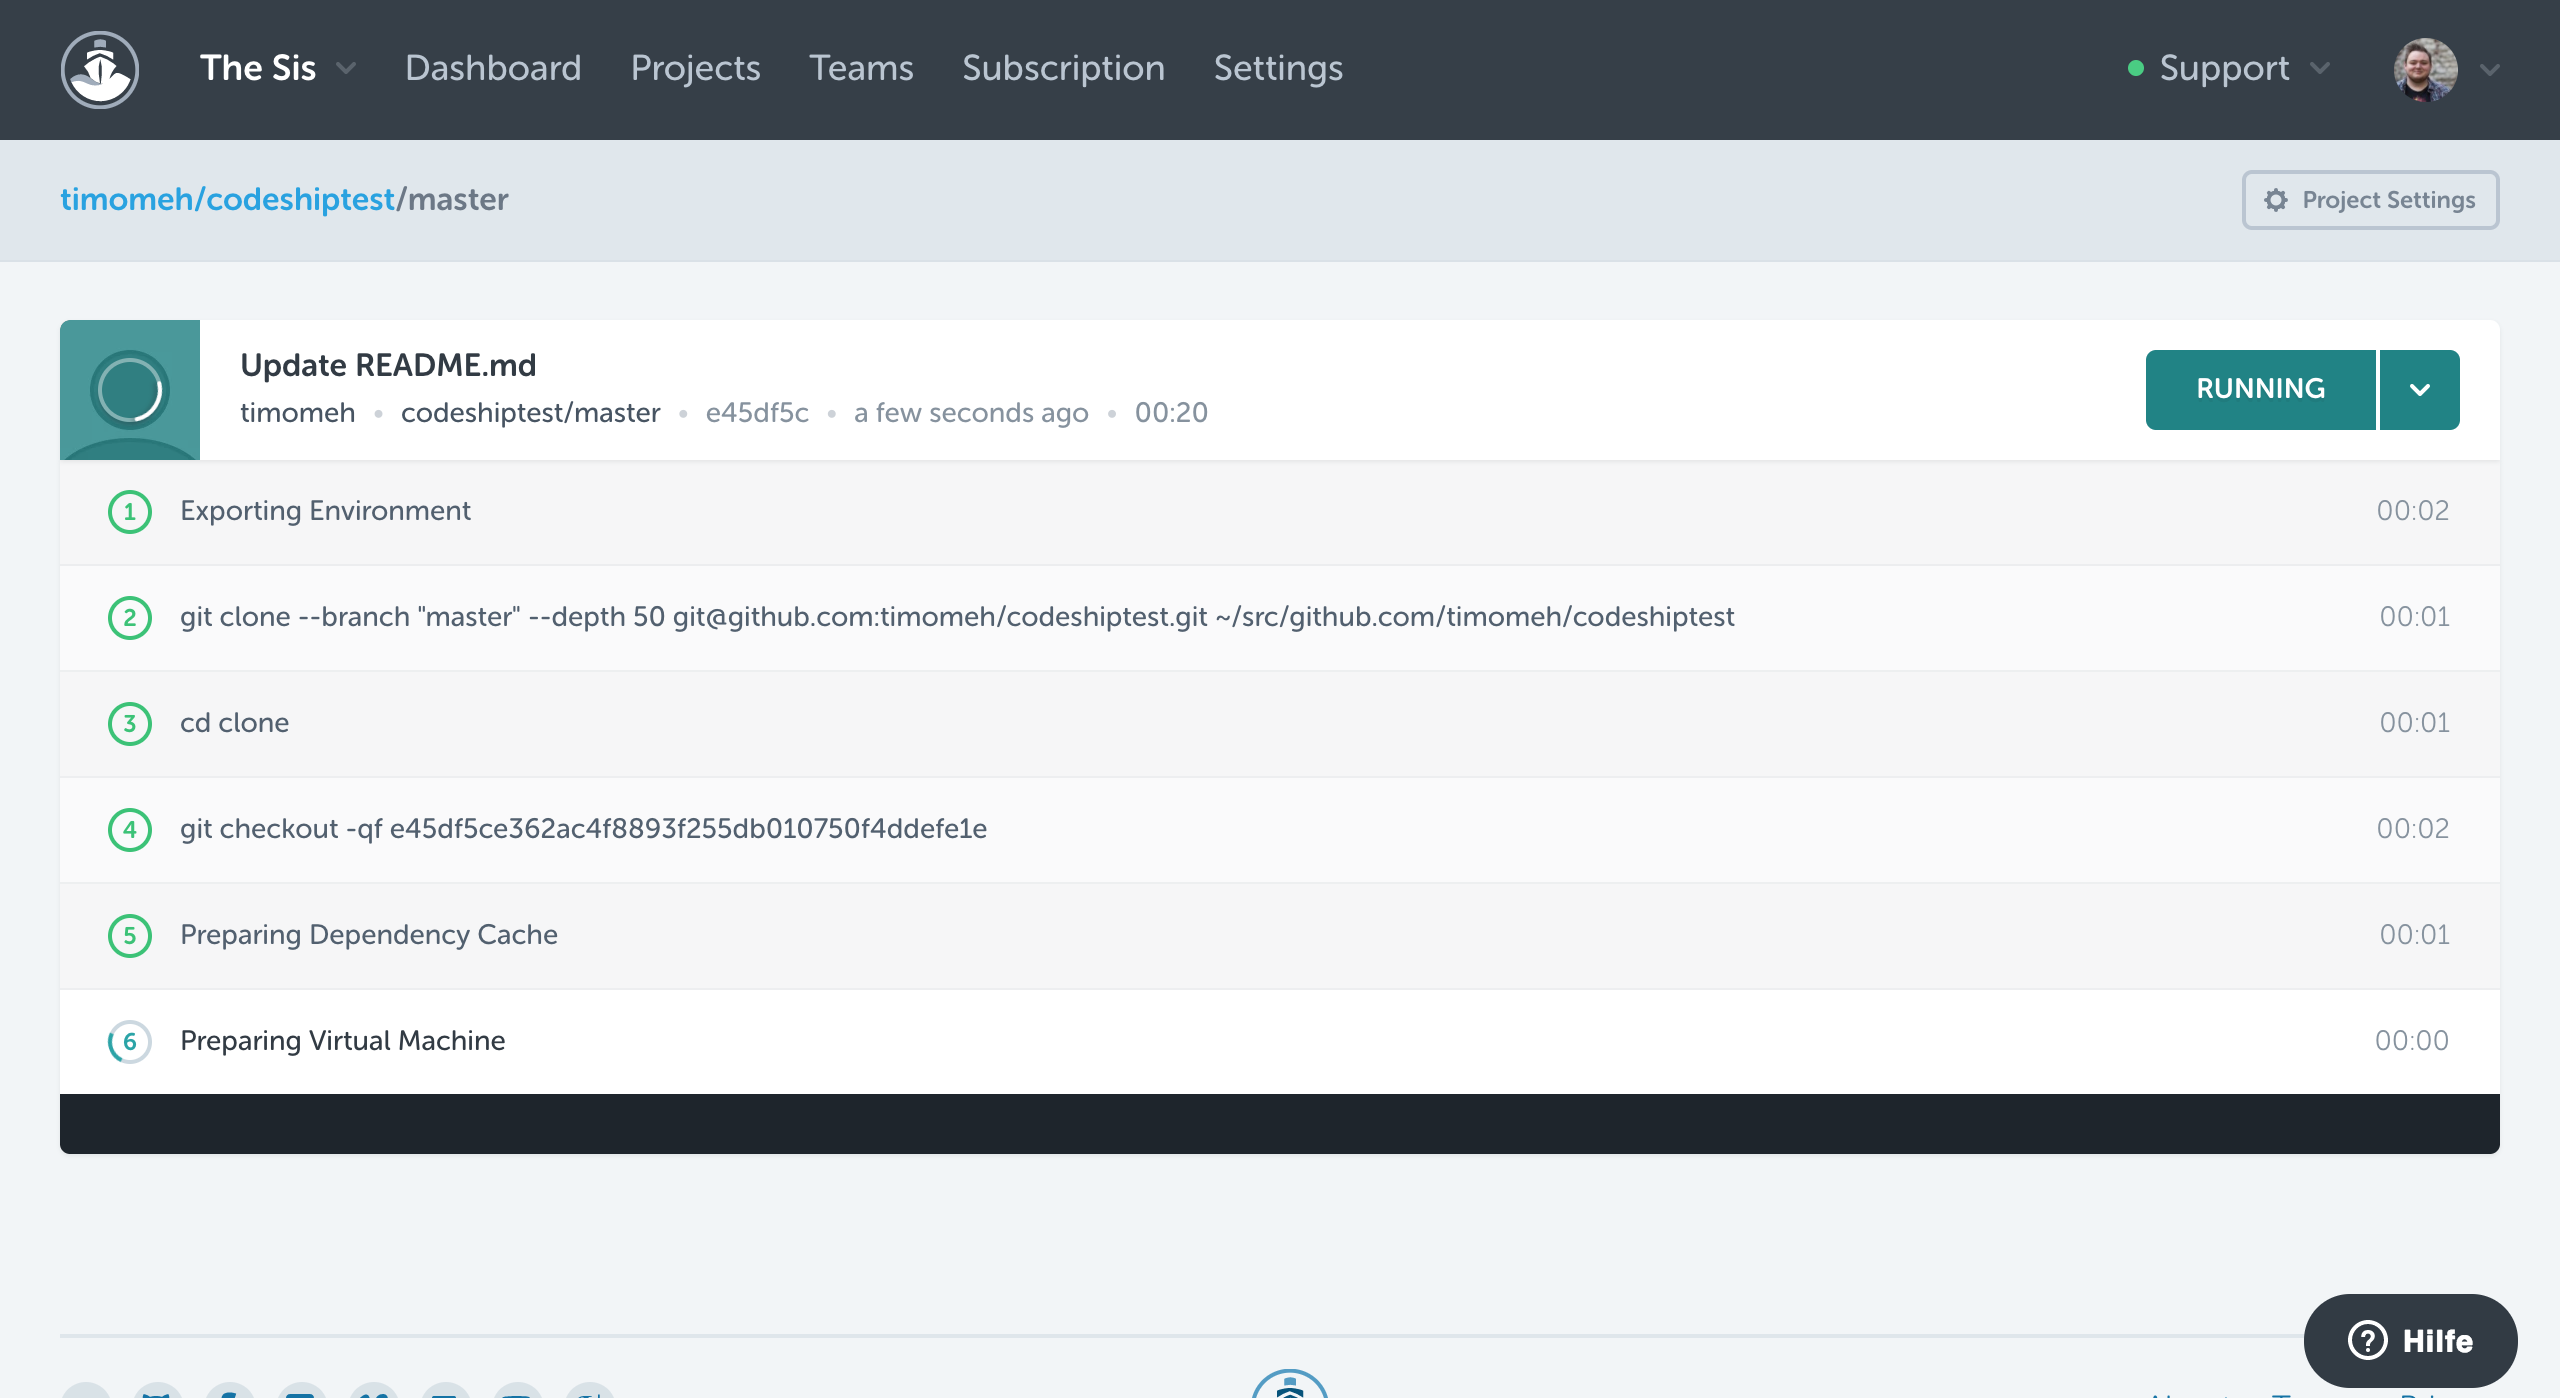
\includegraphics[width=.8\textwidth]{assets/codeship-build-details}
\end{figure}

Codeship nutzt nicht die Struktur mit Stages, sondern nur Schritte, die parallel oder seriell ausgeführt werden.

\subsection*{Vorteile von Codeship}

\begin{itemize}
  \item Modernes Design
  \item Abgrenzung nach Organisation
  \item Grundlegende Funktionen kostenlos verfügbar
  \item Verfügbar für GitHub, Bitbucket und GitLab
\end{itemize}

\subsection*{Nachteile von Codeship}

\begin{itemize}
  \item Viele Funktionalitäten nur gegen Aufpreis verfügbar, auch bei öffentlichen Projekten
  \item Keine Übersicht nach Branches
  \item Builds können nicht zeitgesteuert gestartet werden
  \item Keine Struktur nach Stages
\end{itemize}
